\documentclass[12pt,oneside]{uhthesis}
\usepackage{subfigure}
\usepackage[ruled,lined,linesnumbered,titlenumbered,algochapter,spanish,onelanguage]{algorithm2e}
\usepackage{amsmath}
\usepackage{amssymb}
\usepackage{amsbsy}
\usepackage{caption,booktabs}
\captionsetup{ justification = centering }
%\usepackage{mathpazo}
\usepackage{float}
\setlength{\marginparwidth}{2cm}
\usepackage{todonotes}
\usepackage{listings}
\usepackage{xcolor}
\usepackage{multicol}
\usepackage{graphicx}
\floatstyle{plaintop}
\restylefloat{table}
\addbibresource{Bibliography.bib}
% \setlength{\parskip}{\baselineskip}%
\renewcommand{\tablename}{Tabla}
\renewcommand{\listalgorithmcfname}{Índice de Algoritmos}
%\dontprintsemicolon
\SetAlgoNoEnd

\definecolor{codegreen}{rgb}{0,0.6,0}
\definecolor{codegray}{rgb}{0.5,0.5,0.5}
\definecolor{codepurple}{rgb}{0.58,0,0.82}
\definecolor{backcolour}{rgb}{0.95,0.95,0.92}

\lstdefinestyle{mystyle}{
    backgroundcolor=\color{backcolour},   
    commentstyle=\color{codegreen},
    keywordstyle=\color{purple},
    numberstyle=\tiny\color{codegray},
    stringstyle=\color{codepurple},
    basicstyle=\ttfamily\footnotesize,
    breakatwhitespace=false,         
    breaklines=true,                 
    captionpos=b,                    
    keepspaces=true,                 
    numbers=left,                    
    numbersep=5pt,                  
    showspaces=false,                
    showstringspaces=false,
    showtabs=false,                  
    tabsize=4
}

\lstset{style=mystyle}

\title{Detección de baches}
\author{\\\vspace{0.25cm}Javier E. Domínguez Hernández\\\vspace{0.2cm} David Orlando De Quesada Oliva}
\advisor{\\\vspace{0.25cm}Yudivián Almeida\\\vspace{0.2cm}Carlos Bermudez Porto}
\degree{Licenciado en (Matemática o Ciencia de la Computación)}
\faculty{Facultad de Matemática y Computación}
\date{Fecha\\\vspace{0.25cm}\href{https://github.com/username/repo}{github.com/username/repo}}
\logo{Graphics/uhlogo}
\makenomenclature

\renewcommand{\vec}[1]{\boldsymbol{#1}}
\newcommand{\diff}[1]{\ensuremath{\mathrm{d}#1}}
\newcommand{\me}[1]{\mathrm{e}^{#1}}
\newcommand{\pf}{\mathfrak{p}}
\newcommand{\qf}{\mathfrak{q}}
%\newcommand{\kf}{\mathfrak{k}}
\newcommand{\kt}{\mathtt{k}}
\newcommand{\mf}{\mathfrak{m}}
\newcommand{\hf}{\mathfrak{h}}
\newcommand{\fac}{\mathrm{fac}}
\newcommand{\maxx}[1]{\max\left\{ #1 \right\} }
\newcommand{\minn}[1]{\min\left\{ #1 \right\} }
\newcommand{\lldpcf}{1.25}
\newcommand{\nnorm}[1]{\left\lvert #1 \right\rvert }
\renewcommand{\lstlistingname}{Ejemplo de código}
\renewcommand{\lstlistlistingname}{Ejemplos de código}

\begin{document}

\frontmatter
\maketitle

\begin{dedication}
    " \emph{Don't fear failure. 
    Not failure, but low aim, is the crime.\\ 
    In great attempts it is glorious even to fail.\\}"\\
    \hfill  Bruce Lee
    \newline
    \newline
    \newline
    \newline
    A nuestros padres y profesores, por habernos apoyado en este gran intento.

\end{dedication}
\begin{acknowledgements}
	A los profesores de la facultad, por encender la llama de la curiosidad en nosotros. Sin la motivación
	que ellos despertaron e inculcaron no hubiera sido posible llegar tan lejos.\\

	A nuestros compañeros de año con los que tantas horas compartimos y con los que tantas notas luchamos.\\


	A los alumnos ayudantes que, a pesar de no ser profesores, compartieron su pasión y su conocimiento con 
	nosotros.\\

	A nuestro tutor Yudivián, por acogernos desde el principio y por guiarnos a pesar de las dificultades.\\


	A nuestros padres y otros familiares, por apoyarnos en este largo viaje a pesar de todo.\\


	Y a todos aquellos que, de una forma u otra, nos impulsaron a continuar y llegar hasta aquí.
\end{acknowledgements}

\begin{opinion}
    Los estudiantes Javier E. Domínguez y David O. De Quesada Oliva desarrollaron satisfactoriamente el trabajo de diploma titulado 
    “Enfoque de Machine Learning para la Detección de Baches”. En este trabajo los estudiantes propusieron un sistema para 
    la detección automática de baches en la carretera.

    La propuesta que presentan se basa en las señales que generan los sensores de un dispositivo móvil (en particular, el acelerómetro, 
    el giroscopio y el GPS) en un vehículo en movimiento. Para ello, una vez obtenida esta señal se detectan, utilizando diferentes algoritmos, 
    las anomalías que pueden ser catalogados como baches. Luego, a partir de un corpus también confeccionado por los estudiantes, 
    utilizaron algoritmos de aprendizaje de máquina para su clasificación. Posteriormente, realizaron un conjunto de experimentos a 
    partir de un conjuntos de señales capturadas por los estudiantes. Con este ejercicio mostraron la viabilidad de su propuesta.


    Para poder afrontar el trabajo, los estudiantes tuvieron que revisar literatura científica relacionada con la temática así como soluciones 
    existentes y bibliotecas de software que pueden ser apropiadas para su utilización. Todo ello con sentido crítico, determinando 
    las mejores aproximaciones y también las dificultades que presentan.

    Todo el trabajo fue realizado por los estudiantes con una elevada constancia, capacidad de trabajo y habilidades, tanto de gestión, como 
    de desarrollo y de investigación. 

    Por estas razones pedimos que le sea otorgada a los estudiantes David O. De Quesada Oliva y Javier E. Domínguez la máxima calificación y, 
    de esta manera,  puedan obtener el título de Licenciado en Ciencia de la Computación.


\end{opinion}
\begin{resumen}
	Desde hace años, la cantidad de personas con dispositivos móviles ha crecido de manera vertiginosa. El desarrollo
	tecnológico ha permitido que dicha tecnología llegue a cada vez más personas a nivel mundial y facilite ciertas actividades 
	de la vida cotidiana del ser humano. Acá en Cuba, el incremento de usuarios de dispositivos móviles ha sido notable en los últimos
	años, más aún desde la aparición de los datos móviles. Por otro lado, el mal estado de las carreteras en La Habana, sigue siendo un 
	tema complejo, al que no se le ha encontrado solución definitiva. Es en este problema, donde el mencionado incremento de dispositivos
	móviles en el país puede representar un posible factor que contribuya de alguna forma a solucionarlo. Estos dispositivos poseen 
	sensores integrados que permiten recopilar información que puede ser útil para monitorear el estado de la carretera de forma sencilla y 
	barata. Muchos autores en la literatura han propuesto varios métodos para llevar a cabo esta tarea, desde técnicas basadas en umbrales 
	hasta los más reciente enfoques utilizando aprendizaje de máquinas. En este trabajo se propone explorar la factibilidad
	de una propuesta, utilizando modelos de aprendizaje de máquina, para detectar baches en la carretera. Estos modelos utilizan características 
	generadas a partir de los datos recopilados con los sensores integrados de los dispositivos móviles, específicamente el
	\textbf{acelerómetro}, \textbf{giroscopio} y \textbf{GPS}. De esta forma, se abrió una línea de investigación que puede ser enriquecida
	y mejorada con futuros trabajos, y que tiene como meta final lograr una plataforma que pueda facilitar el monitoreo del estado de las
	carreteras en el país.
\end{resumen}

\begin{abstract}
	In recent years, the number of people with mobile devices has grown at a dizzying rate. Technological development has allowed
	said technology to reach to more and more people worldwide and facilitate certain activities of the daily life of the human
	being. Here in Cuba, the increase in device users mobile phones has been notable in recent years, even more so since the
	appearance of mobile data. On the other hand, the poor condition of the roads in Havana continues to be a complex issue, to
	which no definitive solution has been found. It is in this problem, where the aforementioned increase in mobile devices in
	the country can represent a possible factor that contributes in some way to solving it. These devices have integrated
	sensors that allow the collection of information that can be useful to monitor the state of the road in a simple and cheap
	manner. Many authors in the literature have proposed several methods to carry out this task, from threshold-based techniques
	to the most recent approaches using machine learning. This paper proposes to explore the feasibility of a proposal, using
	machine learning models, to detect potholes in the road. These models use features generated from data collected with the
	built-in sensors of mobile devices, specifically the \textbf{accelerometer}, \textbf{gyroscope} and \textbf{GPS}. In this way,
	a line of research was opened that can be enriched and improved with future work, and which has as its final goal to achieve a
	platform that can ease the monitoring of the state of roads in the country.
\end{abstract}

\tableofcontents
\listoffigures
\listoftables
% \listofalgorithms
% \lstlistoflistings

\mainmatter

\chapter*{Introducción}\label{chapter:introduction}
\addcontentsline{toc}{chapter}{Introducción}

Cuba se ha propuesto, desde hace unos años, llevar a cabo un profundo proceso de informatización.
Entre los temas dentro de dicho proceso que tienen como objetivo facilitar muchas actividades
cotidianas se encuentran: transacciones bancarias, comercio electrónico, mayor acceso a internet, digitalización
de información, acceso a información, etc. A este proceso se le suma el monitoreo de las carreteras, 
el acceso público de las rutas principales de muchos medios de transporte y el conocimiento del tráfico vehicular
que existe en las principales ciudades.

Las carreteras tienen un papel importante parar el desplazamiento 
de personas o mercancías de un lugar a otro. Estas se deterioran debido al clima, al tráfico o a la mala calidad de 
los distintos tipos de trabajo que se llevan a cabo en la vía pública. En Cuba es algo bastante común que la mayoría de 
las carreteras en las grandes ciudades, como La Habana, estén en malas condiciones (ver figura \ref{fig:1}). 
La funcionalidad que debe ofrecer la red de carreteras de un país es crucial para la seguridad y comodidad de las personas. 
De ahí la importancia que tiene la gestión del deterioro de las mismas. La computación ha sido una herramienta muy usada 
para tratar esta situación. Una de las aplicaciones que se le ha dado es predecir el nivel de deterioro que sufrirán 
las carreteras con el tiempo.  

% como, por ejemplo, para predecir el nivel de deterioro que sufrirán con el tiempo.  
% Una de las tantas actividades que desde hace ya tiempo se ha convertido en
% cotidiana, es el uso de los medios de transporte terrestres para desplazar mercancías o personas de un lugar a otro de
% manera más rápida. Para esto se han ido desarrollado las carreteras, y se han ido mejorando con materiales para facilitar
% el desplazamiento y a la vez hacerlas más resistentes.
% Aún así, en los tiempos actuales
% Las carreteras se deterioran debido al clima, al tráfico o a la mala calidad de los distintos tipos de trabajo que se llevan a cabo en la vía
% pública. En Cuba es algo bastante común que la mayoría de las carreteras en las grandes ciudades, como La Habana,
% estén en malas condiciones.\\

\begin{figure}[htb]
	\centering
	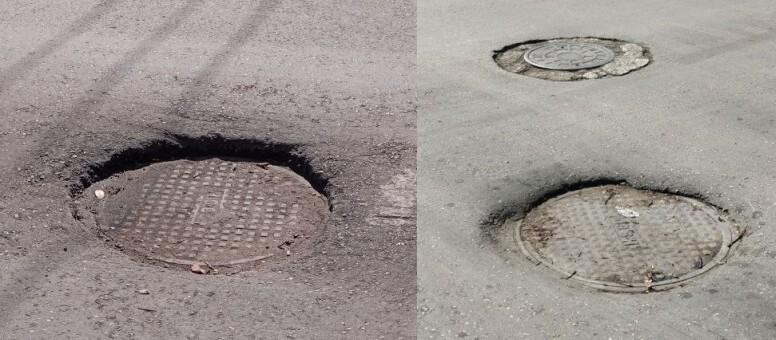
\includegraphics[scale=0.45]{Graphics/pothole_due_to_bad_job_1}
	\caption{Baches ocasionados por trabajos de reparación mal ejecutados.}
	\label{fig:1}
\end{figure}
	
	\subsubsection*{Motivación}
		El acceso rápido a la ubicación de los tramos de carretera en mal estado sería muy útil, pues no solo permitiría agilizar la
		reparación de estas calles, sino que también podría servir de guía a choferes para evitar tales tramos. Esto evitaría las posibles
		consecuencias ocasionadas por estas condiciones, como accidentes y daños a la estructura de los vehículos. Además, el hecho de no tener que
		enviar vehículos a inspeccionar el estado de las carreteras, constituye un ahorro importante de recursos y de tiempo. De esta forma se podrían
		tomar decisiones con mayor rapidez sobre qué tramos de carretera priorizar.
		
		Muchos de los primeros trabajos que se propusieron resolver el problema de determinar los tramos de carreteras en mal estado utilizaban
		métodos de detección que se basaban en fijar umbrales. Estos métodos, a pesar de funcionar, no tenían muy buena precisión\brackcite{eriksson2008pothole,
		mohan2008nericell, mednis2011real}. Más recientemente, con el auge del aprendizaje de máquinas, muchos autores han atacado este problema utilizando
		las bondades de dicha rama, extrayendo varias características de dominio temporal y de frecuencia, y utilizando métodos como \emph{Support Vector
		Machines} (\textbf{SVM}), redes neuronales artificiales(\textbf{ANN}) y árboles de decisión (\textbf{DT})\brackcite{el2018towards, seraj2015roads,
		gonzalez2017learning, zheng2020fused, perttunen2011distributed}. Varios autores han tenido en cuenta, además, la naturaleza contaminada por ruido de
		los datos obtenidos utilizando estos dispositivos y han utilizado técnicas de procesamiento de señales digitales para mejorar la calidad de la señal
		obtenida.  Esto lo realizan con el objetivo de obtener datos más significativos que caractericen de forma más precisa la señal y que, por lo tanto, puedan mejorar
		la calidad de las predicciones de los modelos de \emph{Machine Learning}\brackcite{el2018towards, zheng2020fused, perttunen2011distributed, gonzalez2017learning}.\\
		
	\subsubsection*{Problemática}
		En Cuba no se conoce el uso de alguna forma automatizada de ubicar de manera sencilla y accesible los tramos de carreteras que están en mal estado. 
		Una herramienta que pudiera facilitar esta información podría contribuir a mejorar el estado de los viales en La Habana, y a mantener a las autoridades y a 
		los choferes al tanto de las condiciones de las calles.
		
	\subsubsection*{Hipótesis}
		Para resolver este problema se explorará la factibilidad de un modelo de aprendizaje de máquinas para detectar y clasificar las anomalías en la
		carretera de forma automática. Los datos serán obtenidos de los sensores integrados en un dispositivo móvil, como el \textbf{acelerómetro},
		el \textbf{giroscopio} y el \textbf{GPS}.

	\subsubsection*{Objetivo general y objetivos específicos}
		El objetivo general de este trabajo es proponer un modelo para la detección de baches utilizando los sensores embebidos en los
		dispositivos móviles. Para lograr esto se pretende:

		\begin{itemize}
			\item Estudiar el estado del arte del uso de Dispositivos Móviles para la Detección de Baches.
			\item Determinar el conjunto de sensores apropiados para la detección de baches, así como su frecuencia de muestreo.
			\item Implementar un prototipo de aplicación para la captura de los datos de los sensores, así como la señalización
				manual de baches.
			\item Proponer e implementar un modelo para la detección automática de baches.
			\item Proponer e implementar un prototipo para la visualización de los datos.
			\item Proponer una metodología para validar los resultados parciales.
		\end{itemize}

	\subsubsection*{Propuesta de solución}
		La propuesta en cuestión se basa en los datos que se obtienen con el \textbf{acelerómetro}, el \textbf{giroscopio} y el \textbf{GPS}, que
		son sensores que permiten obtener los datos de la aceleración, la velocidad de giro y la geolocalización del dispositivo móvil respectivamente.
		Con esta información pudiera ser viable implementar un modelo de aprendizaje de máquinas que sea capaz de detectar de forma automática los baches
		en la carretera y ubicarlos en un mapa. Existen varias razones por las que se propone utilizar los dispositivos móviles actuales en la propuesta:\\

		\begin{itemize}
			\item Tener acceso a los sensores de forma independiente es complicado, y lograr una configuración y sincronización de los mismos también lo es.
			\item En la mayoría de los dispositivos móviles estos sensores vienen integrados, lo que facilita la recolección de información.
			\item Cada vez se hace más común que gran parte de las personas tengan un dispositivo móvil y lo usen para realizar distintas actividades.
				Esto permite que sus dispositivos puedan ser utilizados para obtener los datos necesarios a partir de las lecturas que se obtienen de los
				sensores que tienen integrados. Por lo que muchas personas podrían contribuir en la recolección de datos para mejorar la propuesta.
		\end{itemize}

	\subsubsection*{Estructura de la tesis}
		La tesis está estructurada en 3 capítulos. El capítulo 1 es un resumen del estado del arte respecto al problema de la detección de baches en
		la carretera. En este se hace un repaso por los distintos enfoques desde los cuales se ha propuesto resolver dicho problema por varios autores,
		así como de las técnicas más utilizadas. En el capítulo 2 se explica la propuesta desarrollada en esta investigación para detectar baches en la
		carretera mediante el uso de aprendizaje de máquinas. Además, se exponen los sensores que se utilizaron para la recolección de datos, así 
		como los pasos necesarios para poder predecir la presencia de un bache. Finalmente, en el capítulo 3, se explican los detalles 
		de implementación de la propuesta, la aplicación utilizada para la captura de los datos y las tecnologías que permitieron concretar la investigación.
		También se adentra en los experimentos que se realizaron para llevarla  a cabo y hace un análisis de los resultados obtenidos.
		% los experimentos que se realizaron para llevarla  a cabo. Se explica las herramientas que se utilizaron para concretar la investigación y 
		% se analizan los resultados obtenidos.
		
		% dicha propuesta y analizar los resultados.

		% El capítulo 2 contiene la propuesta de solución hecha en esta tesis, donde se explican los detalles de 
		% dicha propuesta.

\chapter{Estado del Arte}\label{chapter:state-of-the-art}

Existen varios artículos científicos que proponen soluciones al problema de identificar cuando hubo una anomalía, algunos proponen métodos
puramente estadísticos y otros utilizan métodos de aprendizaje de máquinas para identificar patrones, mayormente en la serie temporal del
acelerómetro. Entre los varios métodos estadísticos ~\textcite{mednis2011real} propusieron los siguientes:\\

\begin{itemize}
	\item  \emph{\textbf {Z-Thresh}}: Toma el valor del acelerómetro en el eje Z en un instante determinado y compara su valor modular con 
	un valor \emph{threshold} prefijado, si es mayor devuelve \emph{True} indicando que hay una anomalía en ese instante, de lo contrario
	devuelve \emph{False}.\\
	\item \emph{\textbf {Z-DIFF}}: Utiliza el valor del acelerómetro en el eje Z en dos instantes de tiempo consecutivos y compara la
		diferencia modular con un valor \emph{threshold} prefijado, si es mayor devuelve \emph{True} indicando que hay una anomalía en ese
		instante, de lo contrario devuelve \emph{False}.\\
	\item \emph{\textbf {STDEV(Z)}}: Analiza la desviación estándar del valor del acelerómetro en el eje Z durante un intervalo de
		tiempo y compara con un valor \emph{threshold} prefijado, si es mayor devuelve \emph{True} indicando que hay una anomalía en ese
		instante, de lo contrario devuelve \emph{False}.\\ 
	\item \emph{\textbf {G-ZERO}}: Este método se basa en la idea de que cuando el vehículo interactúa con alguna anomalía, existe un
		instante de tiempo donde las lecturas del acelerómetro en los 3 ejes son cercanas a 0 y menores que cierto valor prefijado, lo que
		indica que el vehículo está en caída libre.\\
\end{itemize}

Los 3 primeros métodos requieren información acerca de la orientación del eje Z imaginario del dispositivo encargado de recopilar la información. 
Para capturar datos preliminares utilizaron un collar LynxNet a una frecuencia de 100Hz. Para la evaluación del sistema utilizaron 4 dispositivos
móviles (Samsung i5700, Samung Galaxy S, HTC Desire, HTC HD2), con los que recolectaron más datos y los procesaron con el objetivo de asignar los 
valores óptimos a cada uno de los \emph{threshold}s característicos de cada uno de los 4 métodos propuestos, así como el tamaño de la ventana en caso de 
\textbf {STDEV(Z)}.\\

~\textcite{mohan2008nericell} para el diseño de su estrategia se basaron en 2 ideas, cuando un vehículo interactúa con una
anomalía (un bache en este caso) las ruedas descienden en el hueco ocasionando una caída sostenida en la aceleración en el eje Z,
hasta que alcanzan el fondo del bache y en ese momento se produce un pico bien elevado de aceleración en el eje Z. A altas velocidades
ese pico al final del evento es bien prominente, sin embargo cuando se va a muy poca velocidad no se nota prácticamente, pero la caída
sostenida en la aceleración en el eje Z al entrar al bache si se mantiene, por lo que propusieron 2 métodos para detectar una anomalía
dependiendo de la velocidad $v$ a la que se desplaze el vehículo:\\

\begin{itemize}
	\item \textbf {v > 25 km/h}:  Utilizan un método idéntico al \textbf {Z-THRESH}, o sea, buscan un valor bien prominente de
		aceleración en un instante de tiempo determinado, que sea mayor que cierto \emph{threshold} prefijado.\\
	\item \textbf {v < 25 km/h}:  Utilizan un método que llamaron \textbf {Z-SUS} que busca una caída sostenida en la aceleración
		en el eje Z, por debajo de un cierto \emph{threshold} prefijado, durante cierta cantidad de tiempo.\\
\end{itemize}

Con respecto a los trabajos existentes que utilizan el aprendizaje de máquinas existen varios, ~\textcite{carlos2018evaluation} además de realizar
una comparación de los métodos existentes en su momento, crearon un método en el que utilizaron un enfoque supervisado con \emph{Support Vector Machines} 
(\textbf{SVM}) para entrenar un modelo que decidiera utilizando varios \emph{features} (basados principalmente en la aceleración en el eje Z), sí existía
o no una anomalía. \emph{Features} como la media, desviación estándar, varianza, coeficiente de variaciónn y diferencia entre valor mínimo y máximo. Otros
4 \emph{features} utilizados para otorgar un valor de confianza a 4 de los \emph{features} previamente mencionados excepto a la varianza, comparándolos con
un cierto valor \emph{threshold}. Esta idea fue tomada teniendo en cuenta una serie de artículos con respecto al tema(~\textcite{mednis2011real}), con el
objetivo de mejorar el rendimiento del clasificador. Otro de los \emph{features} es la cantidad de veces que un feature estadístico sobrepasó el valor
\emph{threshold} concebido. Completan los 12 \emph{features} utilizados la suma de los valores de confianza, así como el valor de confianza correspondiente.
Cabe desctacar que implementaron una plataforma llamada Pothole Lab con el objetivo de crear un sitio web público donde tener acceso a data sets robustos y
curados. Los datos que utilizaron fueron obtenidos de este mismo sitio y fueron capturados utilizando un Moto G Android a una frecuencia de 50Hz.\\

~\textcite{seraj2015roads} en su propuesta, incorporaron además los datos del giroscopio con el objetivo de obtener más \emph{features} que permitieran mejorar
la calidad del clasificador. Además, también realizaron un proceso para eliminar el ruido y mejorar la calidad de las señales obtenidas con los sensores de los
dispositivos utilizados para capturar los datos. Separaron las señales en ventanas de 2.5 segundos y extrajeron de ahí varios \emph{features} para el proceso
de entrenamiento. \emph{features} de dominio temporal, \emph{features} de dominio de frecuencia y \emph{features} extraídos de la transformada de wavelet son
los que conforman los vectores. Finalmente entrenaron un modelo utilizando una \textbf{SVM} con los \emph{features} que extrajeron de los datos, razón por la
cual etiquetaron sus datos utilizando vídeos y audios grabados durante la recolección de los datos. El dispositivo que utilizaron para la recolección de los
datos fue un Samsung Galaxy S2 y recopilaron datos a frecuencias de 47Hz y 93Hz.\\

~\textcite{el2018towards} como en el artículo previamente mencionado, llevaron a cabo un extenso proceso, separando las señales de los sensores por
ventanas de 1 segundo y generando vectores de \emph{features} bien extensos en cada una de estas ventanas. Además llevaron a cabo un proceso de eliminación
de ruido de las señales probando varios métodos conocidos en el campo del procesamiento de señales digitales como la transformada de Fourier o la transformada de
Fourier por ventanas discretas (\textbf{WDFT} por sus siglas en inglés), pero finalmente utilizaron transformadas de wavelets para purificar la señales y obtener
datos más confiables con los que llevar a cabo el proceso de entrenamiento del modelo de \emph{Machine Learning}. Se decantaron por un enfoque supervisado, por
lo que etiquetaron de antemano los datos utilizando vídeos capturados durante el mismo proceso de recolección de datos, métodos como \emph{K-Nearest Neighboors}
(\textbf{KNN}), \emph{\textbf{Decision Trees}}, \textbf{SVM} y \emph{ensembles} de clasificadores fueron probados, obteniendo los mejores resultados con las
\textbf{SVM} y los \emph{bagged decision trees}. Utilizaron \emph{features} estadísticos, de dominio temporal, de dominio de frecuencia y de dominio
frecuencia-temporal. Entre los \emph{features} que utilizaron están media, mediana, moda, desviación estándar, varianza, rango entre cuartiles, media de la
frecuencia, la mediana de la frecuencia, etc.\\

% //\\// Pendiente //\\//
% - Añadir detalles sobre el uso del GPS.
% - Añadir detalles sobre si es multi-class classification o binary-classification
% - Añadir detalles sobre el uso de distintos vehículos.
% - Añadir detalles sobre la ubicación de los dispositivos en el vehiculo.

El algoritmo para la detección de anomalías en la carretera propuesto por ~\textcite{eriksson2008pothole} se basa en que condiciones anómalas de la carretera
son reflejadas en características de los datos de aceleración. El problema para identificar baches a partir de lecturas del acelerómetro es bastante
complelejo debido a la amplia variación en las condiciones de la carretera y el comportamiento del conductor. La mayoría de las anomalías pueden ser
caracterizadas como eventos de alta energía en la señal de la aceleración, por si sola la energía de la señal no es suficiente como un criterio de
detección debido a que muchos eventos de alta energía pueden no considerarse anomalías en la carretera. Muchos accesorios de la carretera como
los cruces de trenes, las juntas de expansión, los eventos de alta energía que pueden ser causados por los pasajeros cuando le dan un fuerte
tirón a la puerta del vehículo o si el el conductor frena de manera repentina. Los datos recopilados son divididos en 256 ventanas pues
los eventos que interesan son generalmente eventos de corta duración. Una serie de filtros de procesamientos de señales son aplicados
al  pedazo continuo de ventanas, donde cada filtro está diseñado para rechazar uno o más de un evento que no sea bache.
Las etapas de filtrado se dividen en 5 y son las siguientes:

\begin{itemize}
	\item \emph{\textbf {Velocidad}}: Las ventanas donde el carro no se está moviendo o se está moviendo a muy poca velocidad son ignoradas. 
		De esta forma se rechazan eventos como un tirón en la puerta cuando se baja el pasajero del vehículo.\\
	\item \emph{\textbf {High-pass}}: Los filtros de \emph{high-pass} eliminan las componentes de baja frecuencia de la señal de aceleración en los ejes z y x, 
		que pueden indicar giros, frenazos, etc.\\
	\item  \emph{\textbf {Z-peak}}: Los picos de aceleración en el eje z es la principal característica de las anomalías significativsas de la carretera.
		Este filtro rechaza todas las ventanas con un pico (absoluto) en la aceleración menor que un threshold $t_z$.\\
	\item \emph{\textbf {xz-ratio}}: La aceleración en el eje x puede ayudar a identificar anomalías que abarcan el ancho de la carretera y por lo tanto 
		impactan ambos lados del carro de igual manera.  Asumiendo que el bache solo impacta un lado del carro, un verdadero evento de bache con un
		un gran pico de aceleración en el eje z debería producir un pico significante en el eje x dentro de alguna ventana.\\
	\item \emph{\textbf {speed vs ratio }}:	A altas velocidades, incluso pequeñas anomalías en la carretera pueden crear altos picos en las lecturas 
		de aceleración. Este filtro rechaza ventanas donde el pico de aceleración en el eje z es menor que un factor $t_s$ veces la velocidad a la que 
		va el vehículo.
\end{itemize}

Dado que la frecuencia de captura de la señal del acelerómetro se hace mucho más seguido que la del GPS, proponen estimar la localización del vehículo
cuando ocurra la lectura $l_i$ del acelerómetro usando interpolación lineal entre lecturas de GPS. A pesar que ciertos tipos de anomalías pueden producir
alta energía, no siempre que se produzca esto representa una carretera en mal estado. Los cruces de ferrocarriles, reductores de velocidad y otros
equipamientos bien conocidos embebidos en la carretera pueden producir una alta energía y no se consideran anomalías de la carretera. Para esto proponen
tener una lista negra con los localizaciones de las anomalías que caigan en alguno de estos equipamientos embebidos en la carretera cuya información se
puede obtener de y luego remover los mismos. Debido a que el error en la medición del GPS (alrededor de 5m a la redonda como media) es significativamente
mayor que el tamaño de un bache común, la ausencia de una detección en una localización particular no siempre es un indicativo de que no haya anomalías en
esta []. No es posible determinar puramente por la localización del GPS en el momento en que las ruedas del vehículo hacen contacto con alguna anomalía de
la carretera. Los conductores usuales intentan evitar los baches, por que la probabilidad de detectar una anomalía en la carretera es menor que la que se
debe de esperar de una distribución sin sesgo del área que se intenta mapear.\\

~\textcite{cong2013applying} para la extracción de \emph{features} descomponen la señal usando \textbf{WPD}(\emph{Wavelet Packet Decomposition}) usando
sucesivamente filtros de \emph{low-pass} y de \emph{high-pass}. Donde \textbf{WPD} es llevado a cabo aplicando de forma iterativa filtros espejos en
cuadratura y seguido por submuestreo. La selección de \emph{features} basadas en \emph{Machine Learning} puede ser asistida para reducir la demanda
computacional para la clasificiación. La selección de \emph{features} está diseñada para encontrar las \emph{features} que hacen una mejor discriminación
de los baches y los segmentos normales en estudio. Para la selección de \emph{features} se probaron con cuatro métodos: \textbf{BS}(\emph{Backward Selection}),
\textbf{FS} (\emph{Forward Selection}),  y \textbf{PCA} usando un número diferente de \emph{features} seleccionadas. \textbf{PCA} fue el que
arrojó mejores resultados cuando el número de \emph{features} es mayor que 5, mientras \textbf{FS}(\emph{Forward Selection}) es mejor cuando el número de
\emph{features} es mayor que 2 y menor que 6.\\
Para la clasificicación usaron \textbf{SVM} one-class classification con kernel RBF con parámetros  $\nu = 0.01$  $\gamma = 0.00002$. \textbf{SVM} fué
entrenado con el 70 \%  de los datos (1234 segmentos) y el conjunto de entrenamiento fue escogido de manera aleatoria. El resto de los datos  (530 segmentos)
y en todos los 21 segmentos de anomalías fueron usados para los tests de precisión del modelo \textbf{SVM} construido.\\

~\textcite{kulkarni2014pothole} proponen un sistema que detecta los baches, registra su ubicación, un crea un documento que
puede utilizarse para cargarlo en un servidor centralizado o enviarlo  a las autoridades competentes inmediatamente.  Cuando el usuario inicia su viaje,
lanza la aplicación Android de detección de baches. La aplicación, que tiene como complemento del algoritmo en funcionamiento, detecta los baches en las
carreteras mientras el usuario está conduciendo. Supervisa los cambios en la aceleración. La aplicación añáde la hora actual, las coordenadas geográficas
y las estadísticas de baches al registro de eventos. Cuando el usuario  finalice el recorrido pulsa "Stop"  y se le presenta el registro de eventos. Este
registro debe mantenerse en la base de datos.  El algoritmo que proponen es el siguiente:\\\\
\noindent

\begin{itemize}
	\item  Un filtro de \emph{high-pass} para remover las componentes de baja frecuencia de la señal de aceleración en los eje x y z.  El filtro de \emph{high-pass}
		elimina el desplazamiento de la gravedad. El alpha usado es de 0.8 \\\\
	\begin{align*}
		\alpha = 0.8 \\
		gravity_{x} = \alpha * gravity_x + (1-\alpha) *event.values_{x} \notag\\
		gravity_{y} = \alpha * gravity_y + (1-\alpha) *event.values_{y} \notag\\
		gravity_{z} = \alpha * gravity_z + (1-\alpha) *event.values_{z} \notag\\	
	\end{align*}
			
	Luego el effecto de \emph{high-pass} para la eliminación de las componentes de baja frecuencia
	
	\begin{align*}
		acceleration_{x} =  event.values_{x} - gravity_{x}\\
		acceleration_{y} = event.values_{y} - gravity_{y}\\
		acceleration_{z} = event.values_{z} - gravity_{z}
	\end{align*}

	\item Los picos de aceleración en el eje Z es una de las características principales de las anomalías en la carretera. Este filtro rechaza todas 
	las ventanas con un pico de aceleración en la componente z menor menor que un \emph{threshold} \textbf{tz} ( o sea rechaza la lectura si $accel_z < tz$ ).
	\item Un verdadero evento de bache con una larga aceleración en la componente z debe producir un pico significativo en el eje x. Este filtro rechaza 
	todas las ventanas con un pico de aceleración en la componente z menor que  el producto del \emph{threshold} en el eje x \textbf{tx} por  el pico de aceleración (o sea 
	si tx es el \emph{threshold} en el eje x rechazaría las lecturas que $accel_x < tx * accel_z$).
	\item A altas velocidades pequeñas anomalías pueden crear altos picos en las lecturas de aceleración. Este filtro rechaza las ventans donde los picos de 
	aceleración en el eje z son menores que un factor ts veces la velocidad a la que se viaja(O sea asumiendo que el factor de velocidad es ts, y \emph{speed} la velocidad actual 
	a la que viaje el vehículo rechaza las lecturas que cumplan $accel_z < ts * speed$). 
	\item  Si todas las condiciones anteriores se cumplen entonces se considera un bache o en caso contrario no.
	\item  Se usa una red neural para mejorar la eficiencia y precisión de la detección de baches. Los parámetros de la red neural usados son los siguientes
	\begin{enumerate}
		\item Número de capas de entrada: 3
		\item Input 1 : aceleración en el eje x
		\item Input 2 : aceleración en el eje x
		\item Input 3 : aceleración en el eje x
		\item Número de neuronas ocultas: 6
		\item Número de capas de salidas: 1
		\item Output 1 : Decidir si es un bache
		\item Función de activación: sigmoidal
		\item Algoritmo usado: \emph{backpropagation}
	\end{enumerate}
	
\end{itemize}

~\textcite{zheng2020fused} se refieren a que la mayoría de los artículos con respecto al tema no toman en consideración el hecho que la gran mayoría de la
carreteras que existe en el mundo no posee anomalías, y que la aplicación de técnicas de \emph{Machine Learning} utizando una ventana deslizante a ciegas puede
disminuir considerablemente la precisión y la rapidez del proceso de entrenamiento. Para esto plantean que una anomalía comienza con una señal normal
y luego ocurre un pico de aceleración en el eje Z que excede un \emph{threshold} superior y luego cae y excede un \emph{threshold} inferior o viceversa,
y finalmente la señal vuelve a estabilizarse entre esos dos \emph{threshold}s. Ese intervalo es el que consideran como el intervalo candidato en el que
puede haber una anomalía, y para encontrarlo utilizan primero el método heurístico de establecer un \emph{threshold} superior e inferior en la aceleración
y buscan el primer instante donde la aceleración sobrepasa alguno de los \emph{threshold}s y el último instante, y utilizan un método para encontrar los
instantes de tiempo justo antes de que ocurriera el primer evento y el instante de tiempo justo después de que ocurriera el último evento, de esta forma
logran construir una ventana de tamaño dinámico que contiene toda la información acerca de la anomalía, obteniendo como resultado un conjunto de ventanas
con posibles anomalías en la serie temporal. Luego crean un modelo con un \emph{Random forest} utilizando algunos \emph{features} estadísticos de cada una
de las ventanas para filtrar ventanas que no constituyen anomalías reales, también proponen tratar al vehículo como un modelo de vibración de un nivel de
libertad para lo cual diseñan varios experimentos. Como resultado de esto llegaron a la conclusión de que la varianza de la aceleración en el eje Z cuando
el vehículo interactúa con una anomalía tendrá una relación casi lineal con la profundidad o altura de la anomalía. Utilizando \textbf{KNN} y \textbf{DTW}
(\emph{Dynamic Time Warping} que se utiliza para determinar similitud entre 2 series temporales que puedan ser obtenidas a distintas velocidades), es que
llevan a cabo el proceso de identificar los tipos de anomalías. Los autores comparan su propuesta con otras hechas en los últimos 3 años obteniendo un mejor
\emph{F1 score} al identificar los 3 tipos de anomalías que consideraron en cada uno de los 3 \emph{datasets} que probaron.\\

~\textcite{perttunen2011distributed} explican que los sensores del teléfono móvil son reflejados en las señales de dos maneras: Primero, la señal del
\textbf{GPS} en el teléfono usado tenía muchco ruido. Segundo, las mediciones del \textbf{GPS} y de la aceleración fueron contaminadas por ráfagas,
que son mediciones registradas con la misma marca de tiempo. A continuación, se realizó el rechazo de valores atípicos de GPS y se aplicó el filtro de
Kalman a la latitud y la longitud para reducir aún más el ruido. Después la velocidad será estimamda por cada par consecutivo de latitud y longitud.
La señal resultante de velocidad fué sobremuestrada y filtrada usando límites físicos razonables para la aceleración del vehiculo. Cuando las estimaciones
de velocidad parecían lo suficientemente suaves, la señal estaba a menudo contaminada por una gran latencia en comparación con la estimación de velocidad
original (ruidosa) y la señal no llegaba a cero en las paradas de los vehículos. Para aliviar este problema se usan dos correcciones. En primer lugar, se
elimina una latencia determinada visualmente de la estimación de velocidad filtrada. En segundo lugar, se aplica una fusión muy sencilla de la aceleración
y la señal de \textbf{GPS}: la varianza de la norma de la aceleración se calculó para la señal de aceleración y se examinó visualmente. Mediante un simple
\emph{threshold} fueron capaces de detectar un segmento de la señal, donde la velocidad del vehículo era cero, o muy cercana a cero. A continuación,
establecieron los segmentos correspondientes de la señal de velocidad en cero y suavizaron la señal utilizando un filtro de Kalman. Los datos fueron
seperados usando una ventana deslizante. Experimentaron con pedazos desde 0.5 segundos hasta 2 segundos, esta escala se consideró aceptable para la tarea de
reconocimiento de anomalías, ya que la duración media de las anomalías era alrededor de 2 segundos. Por cada ventana, se determinaba el por ciento de la
ventana cubierta por anomalías (uno o más juntos). La extracción de características se realiza utilizando ventanas deslizantes de 2 segundos de longitud,
con un deslizamiento de 0.5 segundos. Varias características fueron extraídas de la señal de aceleración: la desviación estándar, la media, la varianza,
\emph{peok-to-peak}, \emph{signal magnitude area}, \emph{3-order autoregressive coeficcients}, \emph{til angles}, la raíz de la desviación cuadrática media.
Los valores absolutos de la correlación de señales entre todas las dimensiones son usados también, ya que se observó visualmente muchas veces todas las
señales de aceleración mostraban similar formas de onda en los segmentos de la anomalía. Se utilizaron características basadas en \emph{Fast Fourier
Transformation(FFT)} para incorporar información de frecuencias específicas. Esto se basó en la suposición de que los baches producirían componentes de
menor frecuencia en comparación a la vibración que se origina en el motor y en la superficie normal de la carretera. La energía \textbf{FFT} se extrajo de
17 bandas de frecuencia para cada dirección de la aceleración y los coeficientes cepstrales de frecuencia de mel en 4 bandas. Se utilizó el algoritmo de
selección de \emph{features} \emph{Backward Selection} para seleccionar el conjunto de \emph{features} óptimo tanto para los que eliminaron la dependecia
de velocidad como para los que no. Usaron un método para remover la dependecia de la velocidad en los \emph{features}. Para clasificar las ventanas, que
representan pequeños segmentos de la carratera, se utilizó SVM con kernel RBF. El clasificador con el mejor g-means medio luego de varias corridas fue
seleccionado. Evaluaron 49 combinaciones de parámetros con \textbf{SVM} usando función de kernal radial (RBF), correspondientes a una rejilla de valores
de los parámetros $\gamma$ y C. Presentaron además un \emph{framework} de visualización para los resultados, parar habilitar la inspección visual de,
por ejemplo, los ejemplos cercanos al borde de las clases.\\

~\textcite{pawar2020efficient} utilizan un dispositivo móvil ubicado en el parabrisas del vehículo para capturar las señales del acelerómetro y el
giroscopio. Con esto construyen un vector de 24 \emph{features} entre los cuales están los valores máximo, mínimo, la desviación estándar y la media
de los 3 ejes del acelerómetro así como los del giroscopio, luego estandarizaron los datos para disminuir el efecto de los \emph{outliers} en los
\emph{features} y permite percibir mejor en un gráfico los picos en las lecturas causados por los baches. Finalmente proponen como modelo una red
neuronal con 2 capas ocultas y 1 capa de salida, cada una de las capas ocultas compuesta de una capa densa con función de activación ReLU, permitiendo
\\emph{backpropagation} de forma más rápida. Adicionalmente cuenta con una capa de \emph{dropout} con el objetivo de prevenir el \emph{overfitting},
asignando 0 como valor de forma aleatoria a un porciento de las entradas luego de cada actualización. La capa de salida tiene como función de activación
la sigmoidal. La función de pérdida es \emph{binary cross entropy} y la red neuronal es entrenada durante 140 épocas con un \emph{batch size} de 3.
Compararon su propuesta con otras similares pero modificando los hiperparámetros e incorporando un modelo conocido como \textbf{SMOTE}(\emph{Synthetic
Minority OverSampling Technique}) con el objetivo de contrarrestar el gran desbalance entre clases que hay en este problema en particular(bache y no
bache en este caso).\\ ~\textcite{gonzalez2017learning} realizaron un riguroso proceso de experimentación con respecto al tipo y total de vehículos con
un total de 12, entre ellos camiones incluidos, además probaron con distintas posiciones del móvil dentro del vehículo. Para la recolección de datos 2
personas iban en el vehículo, uno de ellos encargado de etiquetar las anomalías de la siguiente forma, cuando se van acercando a la anomalía ponen el
dispositivo a recolectar los datos y una vez pasan la anomalía detienen la recolección de datos y asignan una etiqueta a dicha serie temporal. Su
propuesta consiste en una forma distinta de procesar los datos capturados con el acelerómetro del dispositivo móvil, que es utilizando lo que se conoce
como \emph{Bag of Words representation}, donde los datos son representados utilizando un histograma que refleja la cantidad de veces que se repite una
palabra en un documento determinado. Esta representación se ha utilizado en áreas como visión por computadoras, procesamiento del habla y procesamiento
de series temporales como es el caso de este problema en particular. El objetivo es crear un diccionario de palabras clave que describa la serie temporal
por fragmentos (un tamaño prefijado) y luego representar en un histograma la frecuencia con que aparece cada palabra clave en una serie temporal dada.
Para crear esta lista de palabras clave separan en una cantidad de tramos prefijada las series temporales de los datos recolectados y etiquetados, con
datos de estos tramos como las lecturas, la media, la varianza, y los valores máximo y mínimo corren \emph{k-means} con todos los datos de una clase para
cada una de las clases, con el objetivo de agrupar los tramos similares en \emph{clusters} y obtener $k$ centroides, cada uno de estos lo consideran una
palabra clave perteneciente a una de las clases en cuestión. De esta forma cada clase tiene $k$ centroides que son sus palabras clave y así se obtiene 
un diccionario de clase:palabras clave. Luego para construir el vector de \emph{features} segmentan la señal por tramos y comparan cada tramo con cada
uno de las palabras clave en el diccionario utilizando distancia euclideana y asignando a cada tramo la palabra clave con menor distancia, de esta forma
cada tramo se convierte en una palabra clave y es convertido a un histograma donde cada característica constituye la cantidad de veces que se repite cada
palabra clave en esa serie temporal, y es este vector el que entregan al clasificador. Probaron con una gran variedad de clasificadores redes neuronales
artificiales(\textbf{ANN}), \textbf{KNN}, \emph{Naive Bayes}(\textbf{NB}), \emph{Random Forest} (\textbf{RF}), \emph{Decision Trees}(\textbf{DT}),
\textbf{SVM}, y \emph{Kernel Ridge}(\textbf{KR}).\\

\chapter{Propuesta}\label{chapter:proposal}
	La propuesta de solución consiste en varios pasos. Primero se capturan las señales de los sensores y se almacenan.
	Luego, se realiza un preprocesado de los datos, para eliminar datos que sean erróneos. Durante este proceso, también
	se extraen ciertas características importantes a partir de las ya existentes en los datos obtenidos durante la fase
	de captura de señales. Una vez se tengan los datos que se quieren estructurados, se pasa a una fase de detección de
	anomalías utilizando algunos métodos heurísticos y de aprendizaje no-supervisado. Las anomalías que se extraigan con
	este proceso son etiquetadas con un método que utiliza la distancia de la ubicación de las lecturas a ciertas marcas
	previamente etiquetadas a mano. Luego se realiza un proceso de selección de características utilizando varios métodos 
	para determinar las más relevantes a la hora de clasificar las anomalías en bache o no bache. Finalmente, se realiza 
	un proceso de selección de modelos e hiperparámetros, mediante el cual se busca un algoritmoy una configuración de 
	hiperparámetros que maximice el \emph{F1 score}.

\section{Captura de señales}
	Las señales que se consideraron capturar son las proporcionadas por sensores como el \textbf{acelerómetro},
	el \textbf{giroscopio} y el \textbf{GPS}, pues son los sensores más comunes en los teléfonos inteligentes. El
	\textbf{acelerómetro}, como se explica en la literatura, permite medir en tiempo real la aceleración(rapidez de
	cambio de la \textbf{velocidad}) en $m/s^2$ con respecto a los 3 ejes principales, y en el caso de los
	acelerómetros integrados en los teléfonos inteligentes permite medir la aceleración en los 3 ejes
	principales del dispositivo en cuestión. Estos 3 ejes(figura \ref{fig:2}) se encuentran ubicados, si se sostiene el
	dispositivo de la forma usual, de la siguiente manera:

	\begin{itemize}
		\item eje X: Va de un lado del dispositivo a otro (lateral).
		\item eje Y: Va desde la parte inferior hasta la parte superior del dispositivo (longitudinal).
		\item eje Z: Es ortogonal a la pantalla del dispositivo (vertical).
	\end{itemize}
	
	\begin{figure}[htb]
		\centering
		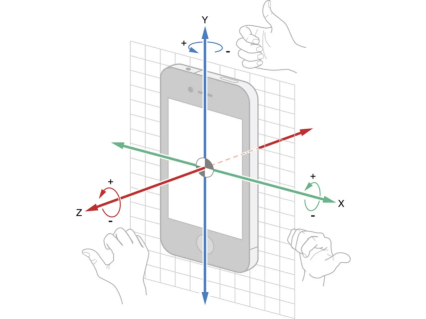
\includegraphics[scale = 0.4]{Graphics/mobile_phone_axis.png}
		\caption{Ejes de un dispositivo móvil}
		\label{fig:2}
	\end{figure}

	Por su parte, los ejes correspondientes a un vehículo(figura \ref{fig:3}) están distribuidos de la siguiente forma:

	\begin{itemize}
		\item eje X: Va de un lado del vehículo a otro (lateral).
		\item eje Y: Va desde la parte trasera hasta la parte delantera del vehículo (longitudinal).
		\item eje Z: Es ortogonal al vehículo, es decir, va desde la parte inferior hasta la parte superior del mismo (vertical).
	\end{itemize}

	\begin{figure}[htb]
		\centering
		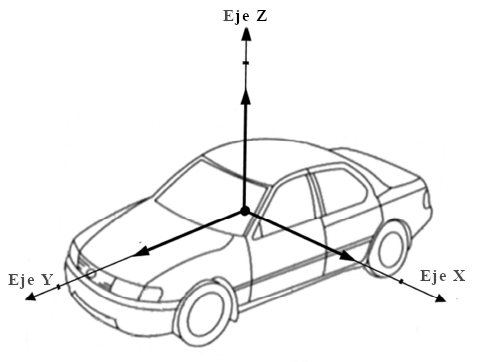
\includegraphics[scale = 0.4]{Graphics/car-axis.jpg}
		\caption{Ejes de un vehículo}
		\label{fig:3}
	\end{figure}

	\subsection{Acelerómetro}
		La señal del \textbf{acelerómetro} mientras el vehículo se desplaza por carreteras en buen estado es bien similar.
		Sin embargo, una vez pasa por encima de un bache ocurre un evento anómalo en el que el vehículo se ve afectado
		por el bache. En ese momento cae brevemente e incluso se inclina momentáneamente hacia un lado (en el caso de un bache
		que afecte una sola rueda). Por esta razón la señal del \textbf{acelerómetro} en un intervalo de tiempo determinado debe tener
		un comportamiento fuera de lo común que permita identificar el evento en la serie temporal capturada por este sensor.\\
		\indent Tal como se plantea en la literatura, la característica fundamental de un bache son lecturas anormales en el eje
		Z del \textbf{acelerómetro} durante un intervalo de tiempo determinado. También, dicho sensor debe registrar lecturas
		anormales en el eje X si el bache afecta un solo lado del vehículo, pues en este caso el vehículo se inclina violentamente
		hacia un lado por un momento(figura \ref{fig:4}).\\

	\begin{figure}[htb]
		\centering
		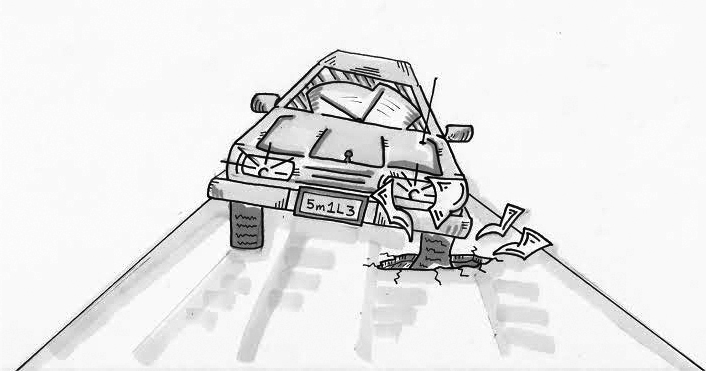
\includegraphics[scale = 0.5]{Graphics/one_side_pothole_vehicle.jpg}
		\caption{Vehículo impactado por un bache en un solo lado}
		\label{fig:4}
	\end{figure}

	\subsection{Giroscopio}
		El \textbf{giroscopio} es otro de los sensores que se considera que aportaría información útil, ya que este sensor 
		mide en $rad/s$ la velocidad angular del dispositivo móvil con respecto a los 3 ejes mencionados previamente. 
		En el momento que un vehículo interactúa con un bache ocurren vibraciones que hacen que el vehículo gire, lo que
		debería generar picos en las lecturas del \textbf{giroscopio} en un intervalo de tiempo. El problema con este sensor es 
		que, a pesar de ser de los más comunes, no es abundante en teléfonos inteligentes de gama baja por lo que 
		su uso en la propuesta de solución se tiene pensado como algo que permita mejorarla y no algo de lo que esta
		dependa.\\

	\subsection{GPS}
		El \textbf{GPS}(\emph{Global Positioning System}) es el sensor que le permite al dispositivo móvil ubicarse sobre la
		superficie de la tierra utilizando coordenadas de latitud-longitud. Debido a que este sistema utiliza señales para
		comunicarse con satélites en tiempo real, existe una latencia debido al tiempo que le toma a la señal viajar hacia el
		satélite y de vuelta al dispositivo. Además, las condiciones atmosféricas pueden afectar esta latencia, así como el hecho
		de que la señal puede ser reflejada por el terreno, edificios, etc., como por ejemplo, cuando se viaja a través de un
		túnel subterráneo donde la señal no puede llegar.\\
		\indent También es importante destacar que las lecturas que genera el \textbf {GPS} tienen cierto margen de error que varía
		de un dispositivo a otro y que depende de la potencia del sensor en sí. En general, según la literatura, la mediana del error
		en estos sensores es de 5m aproximadamente\brackcite{eriksson2008pothole}, ambos aspectos son importantes a tener en cuenta
		al hacer uso de este sensor. El mismo se puede utilizar para estimar la \textbf{velocidad} a la que viaja el vehículo, lo que
		es necesario ya que la \textbf{velocidad} es un factor que influye de forma directa en la forma que un vehículo es afectado por
		un bache. Además, con este sensor es posible ubicar en un mapa, aproximadamente, los lugares donde existen baches u otro tipo
		de anomalías, incluso puede ser útil para marcar rutas de viaje y así facilitar algunos aspectos de la propuesta de solución.

	\subsection{Velocidad y frecuencia de muestreo}
		Debido a que la \textbf{velocidad} de un vehículo durante un recorrido no suele ser constante, es necesario que la \textbf
		{frecuencia de muestreo} del \textbf{acelerómetro} y el \textbf{giroscopio} cambie en función de la \textbf{velocidad}
		a la que vaya el vehículo. Pues si el vehículo se desplaza más rápido será necesario muestrear más para mantener la
		precisión y consistencia de los datos que se generen.\\
		\indent La frecuencia de muestreo se tomó de tal forma que se tuviera una lectura de \textbf{acelerómetro} y \textbf
		{giroscopio} por cada metro. Si el vehículo se desplaza a una \textbf{velocidad} $v$ en $m/s$ y se quiere obtener
		$x$ muestras por cada metro, quiere decir que se necesitan obtener $v * x$ muestras, por lo que la frecuencia de muestreo
		necesaria sería de $v * x Hz$. Como se quiere una sola muestra por cada metro la frecuencia de muestreo
		en este caso particular es de $v Hz$. La actualización de la \textbf{frecuencia de muestreo} ocurre cada vez que se recomputa
		la velocidad, lo que se propuso realizar cada 5 segundos debido a la posible latencia inherente del \textbf{GPS} a la hora
		obtener las lecturas.\\
		\indent Para actualizar de forma correcta la \textbf{frecuencia de muestreo} es necesario conocer la \textbf{velocidad}
		a la que viaja el vehículo, o al menos realizar una estimación aceptable de la misma utilizando los sensores de
		los que dispone el dispositivo móvil. Esta estimación se realizó utilizando las lecturas del \textbf{GPS} y se 
		asignaron frecuencias de muestreo teniendo en cuenta los límites de velocidad existentes en la zona urbana donde 
		se llevaron a cabo los experimentos. Debido a que en Cuba existen muy pocas carreteras donde se permita a
		los vehículos desplazarse a más de 100 km/h y también debido a que la mayoría de los vehículos que circulan en
		el país no alcanzan dicha \textbf{velocidad}, se asumió que esta es la máxima a la que podría desplazarse un
		vehículo a la hora de decidir las frecuencias de muestreo de los sensores.\\
		\indent La frecuencia de muestreo del \textbf{GPS} se fijó constante en 1Hz debido a que es necesario tener 
		la ubicación en tiempo real del dispositivo y buena precisión en las lecturas del propio \textbf{GPS}. Además, 
		muestrear más de una vez por segundo no es necesario, pues la distancia entre una lectura y otra no es considerable.\\

	\subsection{Posición del móvil en el vehículo}
		La posición en la que se coloca el dispositivo móvil en el vehículo a la hora de capturar las señales de los sensores es
		relevante. Esto se debe a que es necesario que las lecturas que se obtengan durante el muestreo sean relevantes y representen
		las características de la carretera por la que viaja el vehículo. Para esto, es necesario colocar el dispositivo móvil de tal 
		forma que la dirección del eje Y del vehículo coincida con la del eje Y del móvil, para que las señales que se capturen
		se correspondan con la realidad. De lo contrario se deberían realizar ciertos ajustes utilizando algún método de
		transformación de coordenadas para poder obtener lecturas acertadas, sin importar la posición en la que se coloque
		el dispositivo.

\section{Preprocesamiento de los datos}
	Luego de recolectar los datos, se lleva a cabo un preprocesamiento de los mismos para eliminar o corregir cierto aspectos.
	El primer aspecto de este preprocesamiento es eliminar lecturas donde la precisión del \textbf{GPS} sea mayor que 10 m
	con el objetivo de tener la mayor precisión posible en los datos recopilados.\\
	\indent También, debido a que la frecuencia de muestreo del \textbf{acelerómetro} y el \textbf{giroscopio} es mayor que la del
	\textbf{GPS}, existen varias lecturas consecutivas con un mismo valor de latitud-longitud en ese intervalo de tiempo. Para
	corregir esto se estimaron los valores de latitud-longitud de dichas lecturas utilizando interpolación lineal entre dos lecturas
	de \textbf{GPS} consecutivas.

	\subsection{Extracción de características}
		Durante este proceso, además de corregir y eliminar ciertos datos, también se extrajeron características. Entre ellas,
		algunas estadísticas.  Luego se incorporaron a cada uno de los datos. Estas características se extrajeron con el objetivo
		de tener un juego de datos que brindara más información acerca de la naturaleza del problema, y así, tentativamente,
		mejorar la calidad de la propuesta.\\

		Las características no estadísticas extraídas fueron:\\

		\begin{itemize}
			\item X/Z: Cociente entre la aceleración en el eje X y la aceleración en el eje Z.
			\item MaxZRatio: Cociente entre la aceleración en el eje Z y el máximo valor de aceleración en el eje Z.
			\item MinZRatio: Cociente entre la aceleración en el eje Z y el mínimo valor de aceleración en el eje Z
			\item SpeedVsZ: Cociente entre la velocidad y la aceleración en el eje Z.
		\end{itemize}

		Las características estadísticas extraídas fueron:\\

		\begin{itemize}
			\item MeanDevAccelX: Desviación del valor de la aceleración en el eje X con respecto a la media.
			\item MedianDevAccelX: Desviación del valor de la aceleración en el eje X con respecto a la mediana.
			\item MeanDevAccelY: Desviación del de la aceleración en el eje Y con respecto a la media.
			\item MedianDevAccelY: Desviación del valor de la aceleración en el eje Y con respecto a la mediana.
			\item MeanDevAccelZ: Desviación del valor de la aceleración en el eje Z con respecto a la media.
			\item MedianDevAccelZ: Desviación del valor de la aceleración en el eje Z con respecto a la mediana.
			\item MeanDevGyroX: Desviación del valor del giroscopio en el eje X con respecto a la media.
			\item MedianDevGyroX: Desviación del valor del giroscopio en el eje X con respecto a la mediana.
			\item MeanDevGyroY: Desviación del valor del giroscopio en el eje Y con respecto a la media.
			\item MedianDevGyroY: Desviación del valor del giroscopio en el eje Y con respecto a la mediana.
			\item MeanDevGyroZ: Desviación del valor del giroscopio en el eje Z con respecto a la media.
			\item MedianDevGyroZ: Desviación del valor del giroscopio en el eje Z con respecto a la mediana.
		\end{itemize}

\section{Detección de anomalías}
	Los baches no son más que anomalías en la carretera. Teniendo en cuenta esto, se propuso detectar dichas anomalías utilizando
	2 enfoques. Primero, intentar identificar las anomalías utilizando los métodos heurísticos sugeridos en la literatura basados
	en umbrales. Segundo, emplear algoritmos de aprendizaje de máquinas para detectar anomalías.\\
	\indent Los métodos heurísticos que se utilizaron en la propuesta fueron \textbf{Z-THRESH}, \textbf{Z-DIFF} y \textbf{G-ZERO}.
	Estos solo hacen uso de las lecturas del \textbf{acelerómetro} para determinar la existencia de una anomalía. Por otro lado los
	métodos de aprendizaje de máquinas que se probaron fueron \textbf{DBSCAN}, \textbf{OPTICS} y \textbf{One Class SVM} utilizando 
	6 características, las lecturas de los 3 ejes del \textbf{acelerómetro}, y además las lecturas de los 3 ejes del \textbf{giroscopio}.
	Este último sensor se incluyó pues se consideró que sus lecturas pueden ser significativas a la hora de determinar la existencia de una 
	anomalía. Este proceso de detección de anomalías se aplicó a cada una de las series temporales obtenidas como resultado del muestreo
	de los sensores del dispositivo móvil.

\section{Etiquetado de anomalías}
	Luego de haber detectado las anomalías es necesario llevar a cabo un proceso de etiquetado para poder utilizar los datos en la siguiente
	fase de la propuesta. Para esto se utilizaron las anomalías extraídas de la serie temporal y una lista de marcas. Estas marcas se realizaron
	manualmente a lo largo de la misma ruta con la cual se generaron las series temporales e indican la presencia de un bache en cierta
	ubicación, con coordenadas de latitud-longitud.\\
	\indent Para asignar la etiqueta de bache a una anomalía se busca en un radio predefinido si existe una marca de bache, de lo contrario, se le
	asigna la etiqueta de no bache. Debido a que es imposible determinar exactamente el punto donde el vehículo hizo contacto con el bache
	utilizando el \textbf{GPS}, a causa del error inherente del sensor, este proceso de etiquetado tiene cierto error. Este error puede ocasionar
	que anomalías que no sean baches sean etiquetadas como tal debido a que exista una marca que indique la presencia de un bache en un radio
	cercano a esta.

\section{Selección de características}
	Ya con los datos etiquetados, lo próximo que se propuso fue llevar a cabo un proceso de selección de características utilizando métodos como
	\emph{Forward Selection}, \emph{Backward Selection} y \emph{Recursive Feedback Elimination}. De esta forma, se podrían determinar cuales de las 
	características que posee nuestro juego de datos son mejores para predecir si una anomalía es bache o no bache. Con lo cual se podría determinar
	automáticamente la existencia de un bache en la carretera.

\section{Selección de modelo}
	Una vez se sabe que características son las mejores para predecir si una anomalía es bache o no, se llevó a cabo un proceso de selección de
	modelo. La métrica de evaluación que se escogió fue el \emph{F1 score} porque se consideró que un equilibrio entre \emph{precision} y
	\emph{recall} es más relevante que el \emph{accuracy} para el problema en cuestión. Este proceso de selección de modelo tiene el
	objetivo de determinar entre varios modelos definidos cual obtiene mejor rendimiento con respecto a la métrica seleccionada utlizando los datos
	del problema. Los modelos entre los cuales se propuso escoger son: \textbf{KNN}, árboles de decisión, \emph{Random Forest}, regresión logística y
	\textbf{SVM}.\\
	\indent Junto con este proceso de selección de modelo también se llevó a cabo una selección de hiperparámetros que permita determinar con
	cuales de estos el modelo arroja mejores resultados. Finalmente, se evaluó el rendimiento del modelo analizando el comportamiento de la métrica
	de evaluación en un conjunto de prueba.

\chapter{Detalles de Implementación y Experimentos}\label{chapter:implementation}

\section{Aplicación para la captura de señales}
	Para capturar las señales se utilizó una aplicación implementada en \textbf{Flutter} 2.10.15, con \textbf{dart} 2.16.2.
	Se utilizaron las bibliotecas \textbf{sensors\textunderscore plus} y \textbf{geolocator}, disponibles en \textbf{Flutter} para obtener acceso
	a las lecturas del \textbf {acelerómetro}, \textbf{giroscopio} y \textbf{GPS}. Para comenzar a realizar una captura se aprieta el botón
	de \emph{Start recorder} y a partir de ese momento la aplicación comienza a reflejar los valores que se obtienen de los sensores en la
	interfaz de usuario.\\
	\indent La aplicación muestra en tiempo real las lecturas de los distintos sensores, así como la velocidad en kilómetros por hora (km/h) y la
	duración de la captura que se está realizando en el momento (ver figura \ref{fig:6}).\\
	\indent Cuando se desea detener la grabación se presiona el botón \emph{Stop recorder}. Luego si se quiere exportar dicha grabación se puede
	hacer presionando el botón de \emph{Save record as} e introduciendo el nombre con el que se desea salvar dichar grabación (ver figura
	\ref{fig:7}). De esta forma se puede acceder a todas las grabaciones para posteriormente utilizarlas en el modelo de aprendizaje de máquinas.\\
	\indent Con el botón \emph{Mark anomaly} se pueden realizar marcas, de esta forma se salvan las coordenadas de latitud-longitud en un
	archivo de marcas. La aplicación tiene, además, un mapa donde se pueden visualizar datos de latitud-longitud previamente guardados.
	Estos se pueden cargar en la pestaña del mapa de la aplicación para poder visualizar dichas marcas en el mapa (ver figura \ref{fig:8}).
	De esta forma se pueden marcar los baches y verlos en un mapa.\\
	
	\begin{figure}[htb]
		\centering
		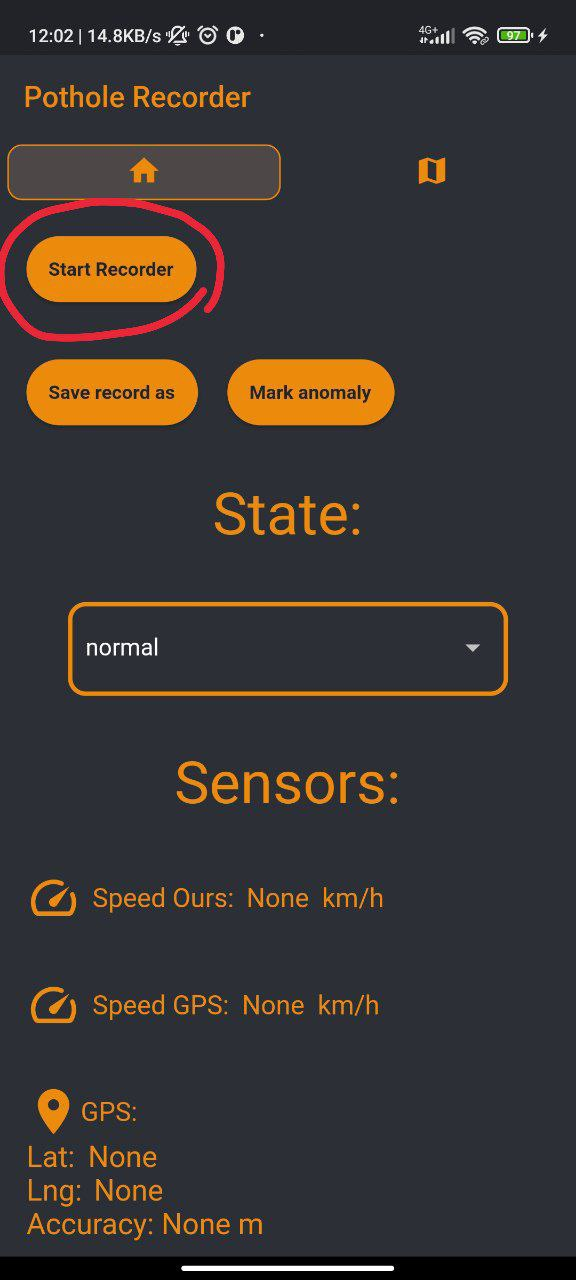
\includegraphics[scale = 0.2]{Graphics/apk_start_recording.jpg}
		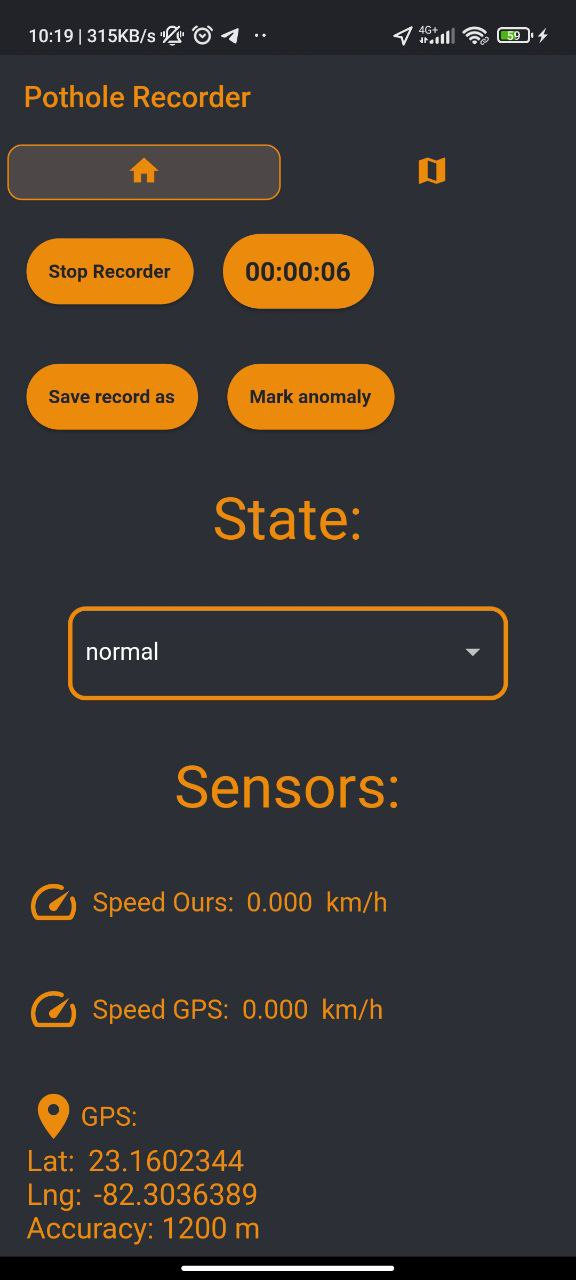
\includegraphics[scale = 0.2]{Graphics/apk_recording_ui.jpg}
		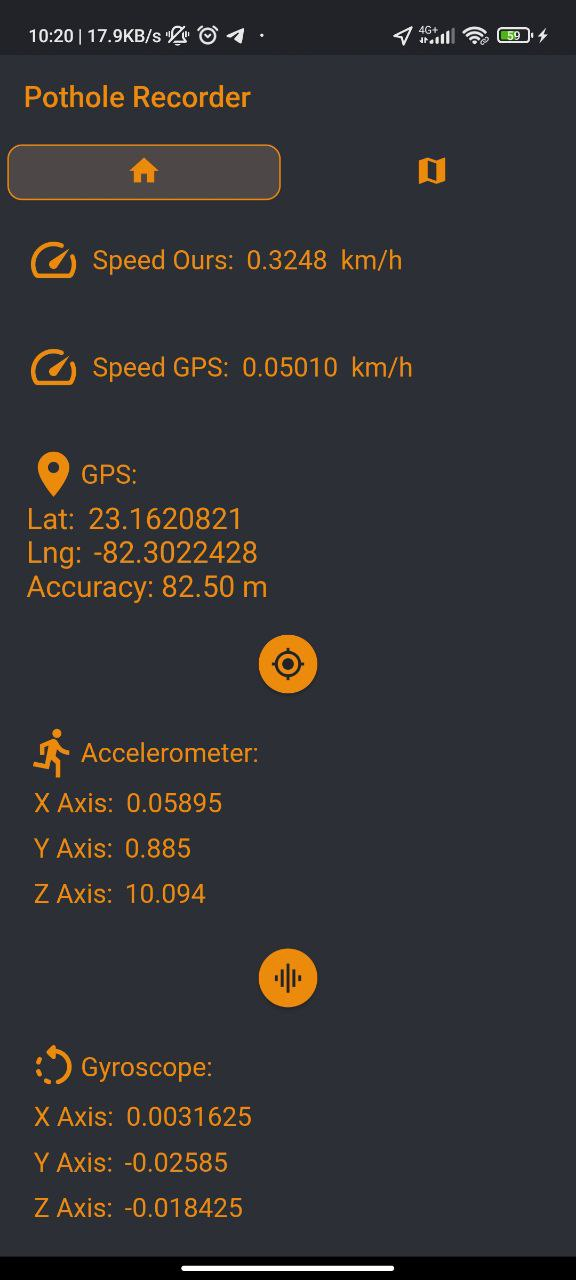
\includegraphics[scale = 0.2]{Graphics/apk_recording_sensors.jpg}
		\caption{Comenzar a grabar y lecturas reflejadas en la aplicación}
		\label{fig:6}
	\end{figure}
	\newpage

	\indent Es necesario dar permisos de escritura para salvar en el dispositivo móvil los archivos que se obtienen como resultado del 
	muestreo de los sensores(los archivos exportados y el archivo donde se almacenan las marcas que se realizan manualmente). Estos archivos
	se guardan en un directorio nombrado \textbf{Baches} en la raíz del almacenamiento interno del dispositivo móvil.\\
	\indent En esta carpeta hay otras 3 carpetas:

	\begin{itemize}
		\item \textbf{mark\textunderscore labels}: Donde se guardan las marcas.
		\item \textbf{sensors}: Donde se guarda el archivo temporal en el que se van guardando los datos que va recopilando la aplicación
			mientras está grabando.
		\item \textbf{exported}: Donde se guardan los archivos exportados.
	\end{itemize}

	Además, es necesario dar permisos de ubicación a la aplicación para que pueda acceder a los datos del \textbf{GPS}, latitud y longitud,
	en tiempo real.

	\begin{figure}[htb]
		\centering
		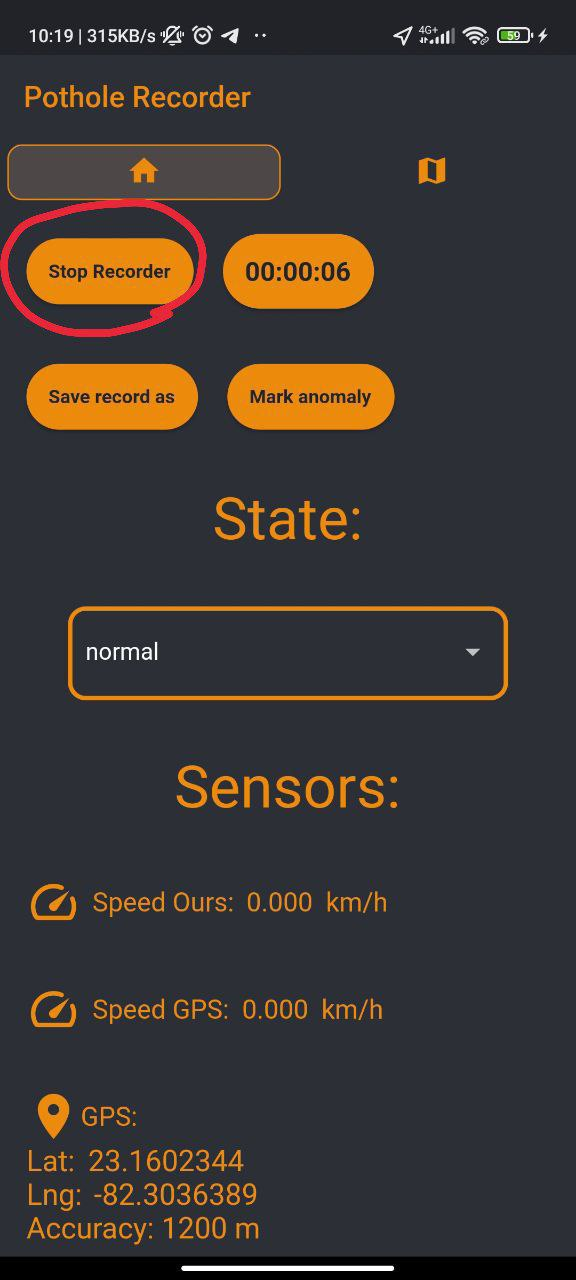
\includegraphics[scale = 0.175]{Graphics/apk_stop_recording.jpg}
		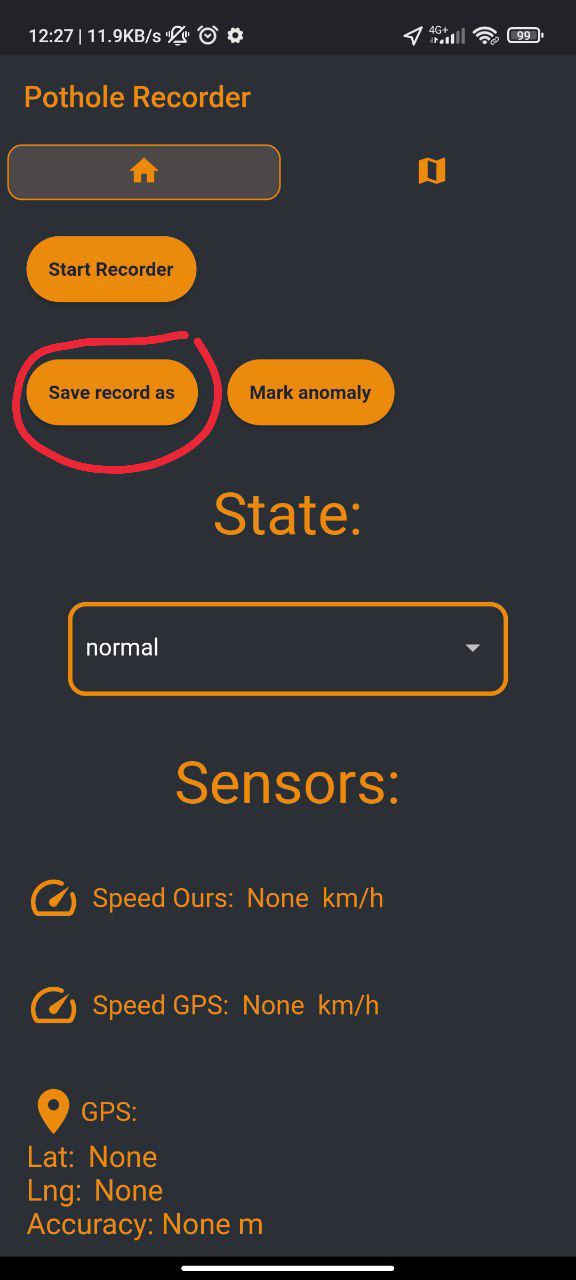
\includegraphics[scale = 0.175]{Graphics/apk_save_recording_1.jpg}
		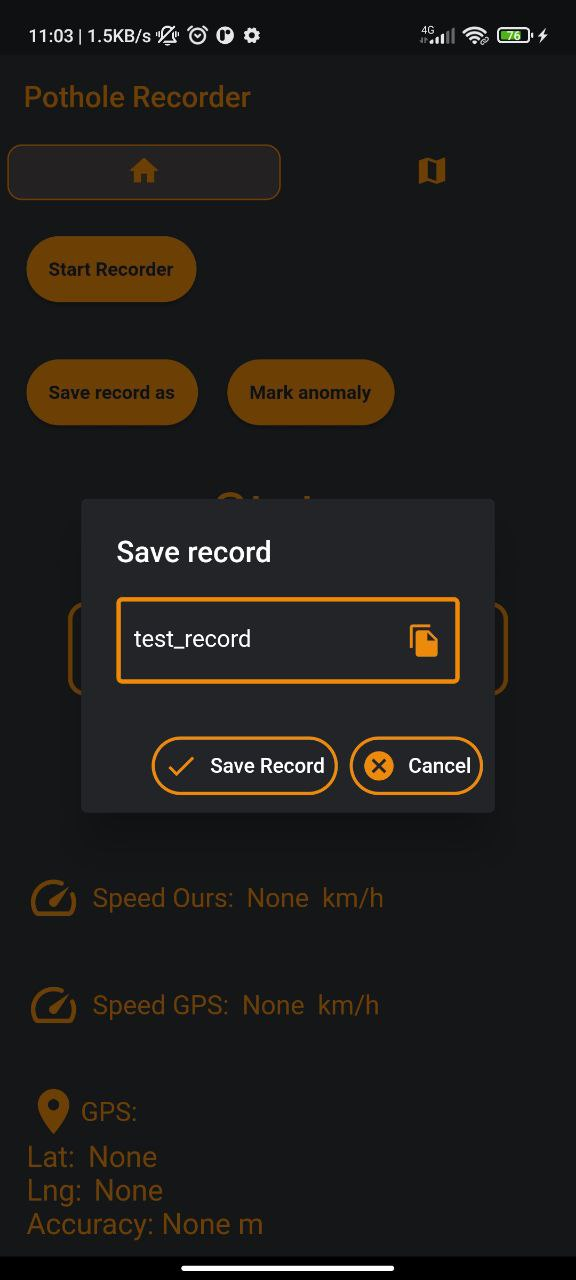
\includegraphics[scale = 0.175]{Graphics/apk_save_recording_2.jpg}
		\caption{Detener grabación y exportar}
		\label{fig:7}
	\end{figure}

	\begin{figure}[htb]
		\centering
		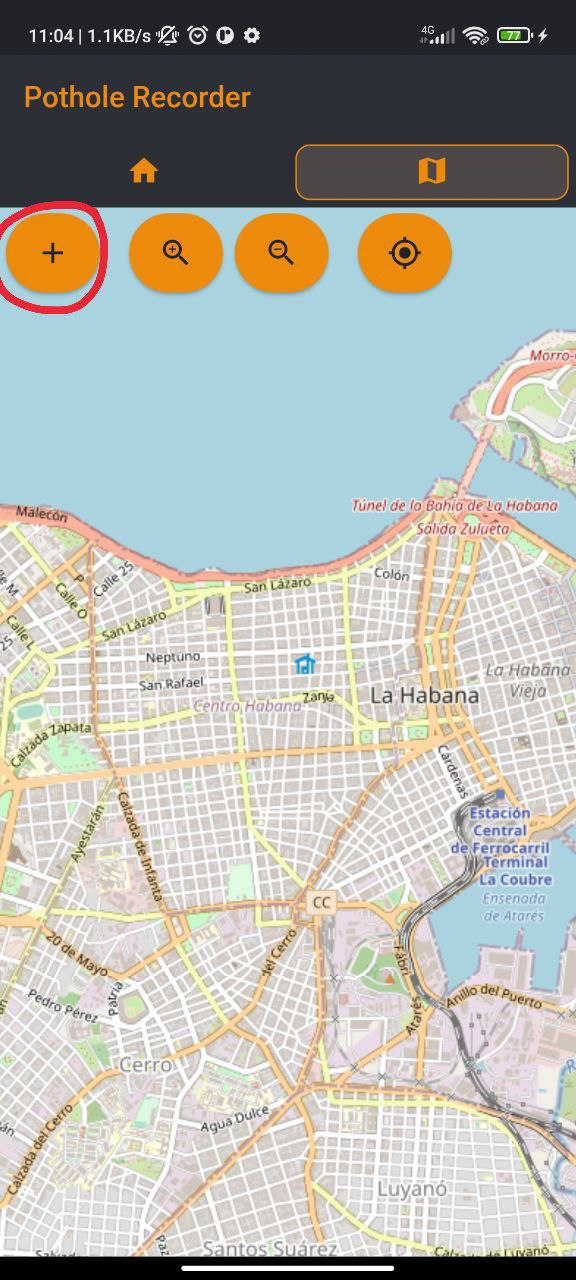
\includegraphics[scale = 0.175]{Graphics/load_marks_to_map_1.jpg}
		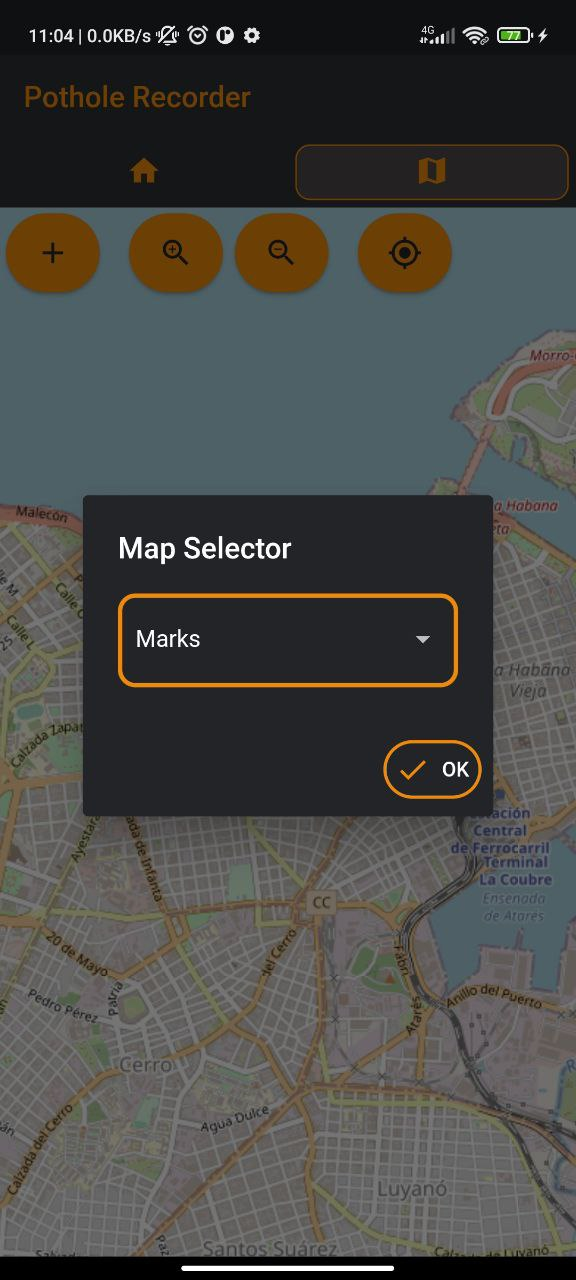
\includegraphics[scale = 0.175]{Graphics/load_marks_to_map_2.jpg}
		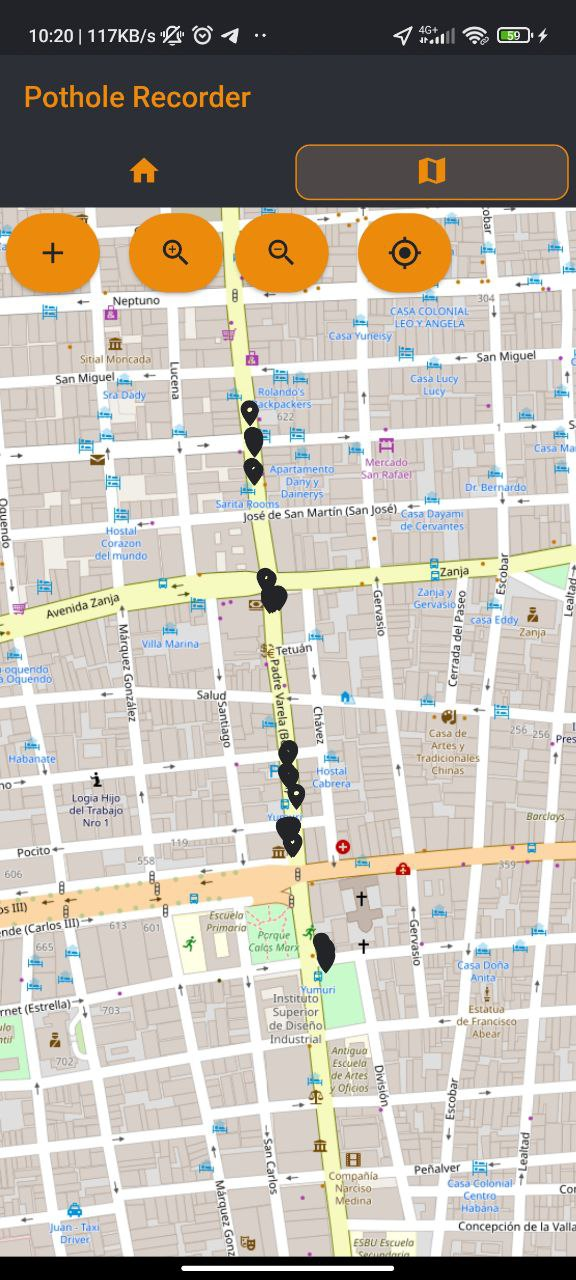
\includegraphics[scale = 0.175]{Graphics/map_marks_apk.jpg}
		\caption{Cargar marcas en el mapa de la aplicación}
		\label{fig:8}
	\end{figure}
	\newpage

	Los datos se guardan en archivos .\textbf{JSON}. Las marcas guardan \textbf{latitud}, \textbf{longitud}, \textbf{precisión} y una 
	etiqueta para indicar que en esa ubicación hay un bache. Por otro lado, las lecturas guardan \textbf{aceleración} en los 3 ejes, 
	\textbf{velocidad de giro} en los 3 ejes, \textbf{latitud}, \textbf{longitud}, \textbf{precisión}, \textbf{velocidad}, \textbf{estado}
	y \textbf{frecuencia de muestreo}. Estos datos se almacenan en el archivo temporal y en los datos una vez exportados. En este último, también 
	se guarda la duración en milisegundos, del recorrido realizado.

	La aplicación cuenta, además, con una funcionalidad que permite etiquetar ciertas capturas con frases como \textbf{girar izquierda},
	\textbf{girar derecha}, \textbf{frenar} y \textbf{normal}. Con estas estiquetas se puede registrar cuando el vehículo dobla en alguna
	esquina o cuando frena mientras se captura la señal. Esto puede ser útil para descartar anomalías asociadas a estos eventos o
	para mostrar y analizar el comportamiento de las señales de los sensores mientras el vehículo se encuentra en alguno de estos estados
	(ver figura \ref{fig:9}).

	\begin{figure}[htb]
		\centering
		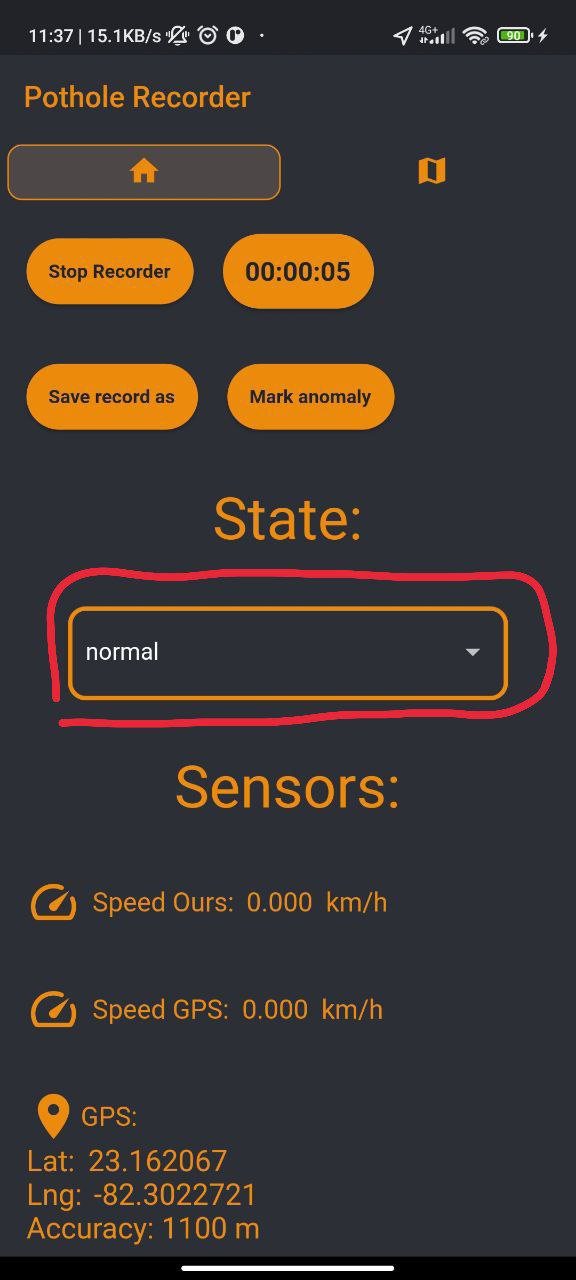
\includegraphics[scale = 0.2]{Graphics/apk_change_state_1.jpg}
		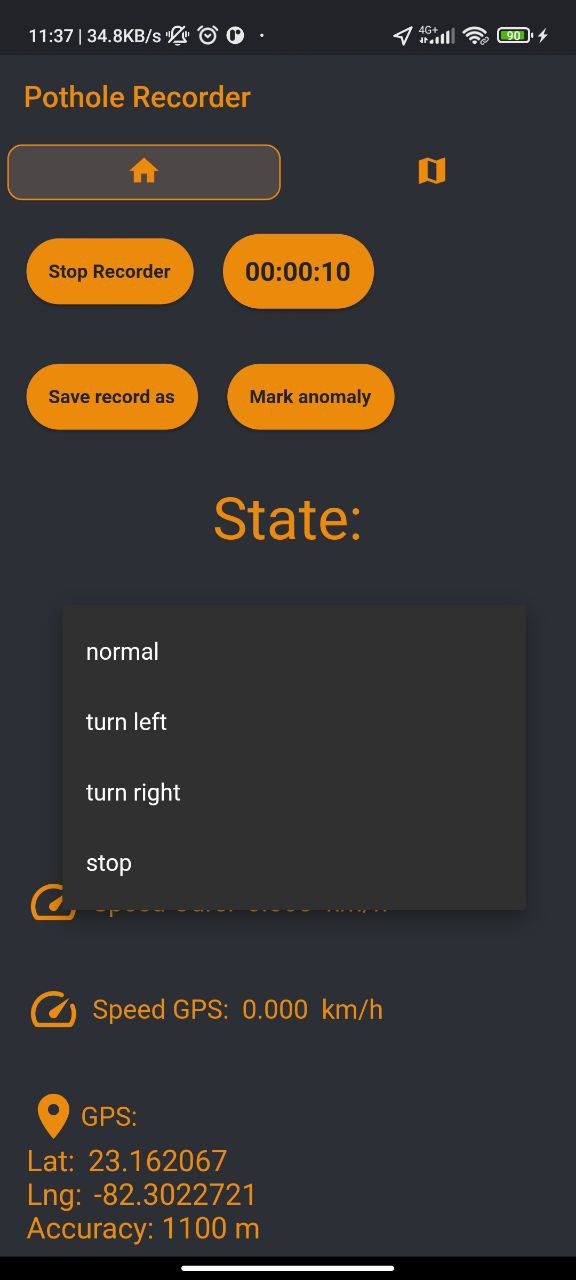
\includegraphics[scale = 0.2]{Graphics/apk_change_state_2.jpg}
		\caption{Cambiar el estado de las lecturas}
		\label{fig:9}
	\end{figure}

	\subsection{\emph{Hardware} y \emph{software} en los que se probó la aplicación}
		La aplicación se probó en dos dispositivos móviles. Un \textbf{Xiaomi Mi A2} y un \textbf{Xiaomi Redmi 10} con \textbf{Android 9} y
		\textbf{11} respectivamente. Ambos dispositivos tienen \textbf{acelerómetro}, \textbf{giroscopio} y \textbf{GPS}. El dispositivo que 
		se escogió para capturar las señales y realizar las marcas de los baches fue el \textbf{Xiaomi Redmi 10}, debido a que este tenía mejor
		precisión en las lecturas del \textbf{GPS}, las cuales se mantuvieron en un rango de 1.3 a 9 metros. En el \textbf{Xiaomi Mi A2}, las 
		lecturas del \textbf{GPS} se mantuvieron generalmente por encima de 50 metros, rara vez por debajo de esa cifra.

	\subsection{Metodología para la captura de señales}
		Primero que todo, para capturar las señales, se escogieron varias rutas de La Habana de longitud moderada. Una vez montado en un vehículo
		se colocó el dispositivo en el asiento de tal forma que su eje Y coindiera con el eje Y del vehículo y su pantalla estuviera hacia arriba.
		Apenas el vehículo comenzó a moverse, se puso la aplicación a grabar. Durante el viaje, dado que no se contaba con un objeto capaz de fijar el
		dispositivo móvil en la posición deseada, se tuvo que sostener lo mejor posible con las manos para que mantuviera la orientación. \\
		\indent Cuando el vehículo se iba a detener por alguna razón y se estaba al tanto, se cambiaba al estado de \textbf{frenar} un poco antes, para
		registrar tal evento en los datos. Lo mismo se hizo cuando el vehículo iba a doblar una esquina. Una vez terminaba el evento, se cambiaba otra
		vez a estado \textbf{normal}. Cuando el vehículo llegaba al final de la ruta planeada, se detenía el proceso de grabación y se exportaban los
		datos de dicho recorrido a un archivo .\textbf{JSON} aparte con un nombre que indentificara la ruta. Se utilizaron dos vehículos para la
		recopilación de los datos: las conocidas \textbf{Gacelas(GAZelles)}, utilizadas como servicio de tranporte de la capital,  
		y un \textbf{Hyundai Atos 1998}.

	\subsection{Metodología para marcar los baches}
		Para marcar los baches, se recorrió la misma ruta que se había seleccionado para capturar los datos y se fueron marcando los baches. Antes 
		de realizar las marcas se esperó un tiempo a que la precisión del \textbf{GPS} se estabilizara en un rango aceptable, preferiblemente por debajo 
		de los 5 metros. Las marcas se realizaron desde la acera debido al tráfico, y en la medida de lo posible un poco más cerca del bache en la calle.
		Por cada bache se realizaron varias marcas con distinta precisión y desde distintas ubicaciones relativamente cercanas a la ubicación real del
		bache con el objetivo de minimizar el efecto del error inherente del \textbf{GPS}. Una vez que se terminaron de marcar los baches en el recorrido
		en cuestión se exportó dicho archivo con un nombre similar al de las lecturas para poder relacionarlos uno con el otro a la hora de utilizarlos.

	\subsection{Error en las lecturas y las marcas}
		En las lecturas durante los recorridos existe cierto error. Esto se debe a que no se pudo fijar el dispositivo en la posición óptima y se tuvo que
		sostener con las manos, lo que sin duda alguna influye negativamente en los datos obtenidos. También en estas lecturas, así como en las marcas, hay un
		error inherente del propio \textbf{GPS}. En las marcas, además, hay un error extra debido a que estas se realizaron desde la acera.

\section{Los juegos de datos}   
	Los juegos de datos que se recopilaron fueron los correspondientes a 3 recorridos hechos a lo largo de 3 rutas de la ciudad de la Habana.

	\begin{figure}[htb]
		\centering
		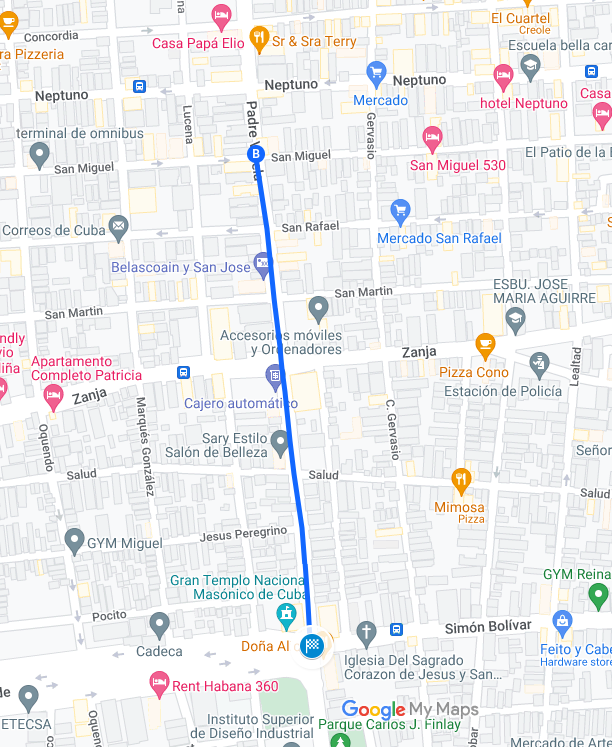
\includegraphics[scale = 0.5]{Graphics/route_1_BelascoainyReina_BelascoainySanMiguel.png}
		\caption{Ruta 1}
		\label{fig:10}
	\end{figure}

	La ruta 1 se tomó empezando en Belascoaín y Reina hasta Belascoaín y San Miguel (ver \ref{fig:10}) y tiene una longitud de 0.5 km. La ruta
	2 comienza en Egido y Arsenal y termina en Ayesteran y 19 de mayo (ver \ref{fig:11}) y tiene una longitud de 3.32 km. La ruta 3 comienza en
	Egido y Arsenal y termina en L y Jovellar (ver \ref{fig:12}) y tiene una longitud de 3.73 km.\\ \indent Se trataron de escoger rutas donde
	hubieran una cantidad importante de baches que se pudieran utilizar para el modelo.
	\newpage

	\begin{figure}[htb]
		\centering
		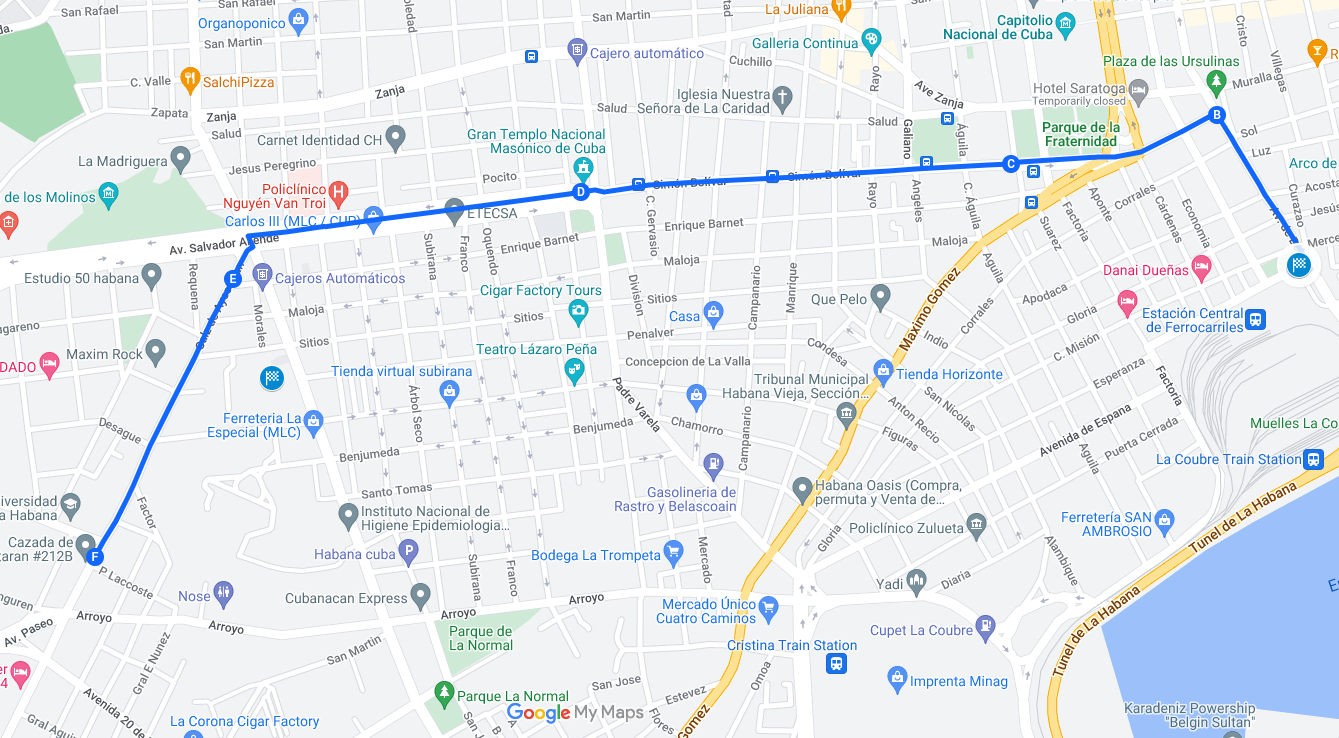
\includegraphics[scale = 0.4]{Graphics/route_2_EgidoArsenal_Ayesteran19deMayo.png}
		\caption{Ruta 2}
		\label{fig:11}
	\end{figure}

	\begin{figure}[htb]
		\centering
		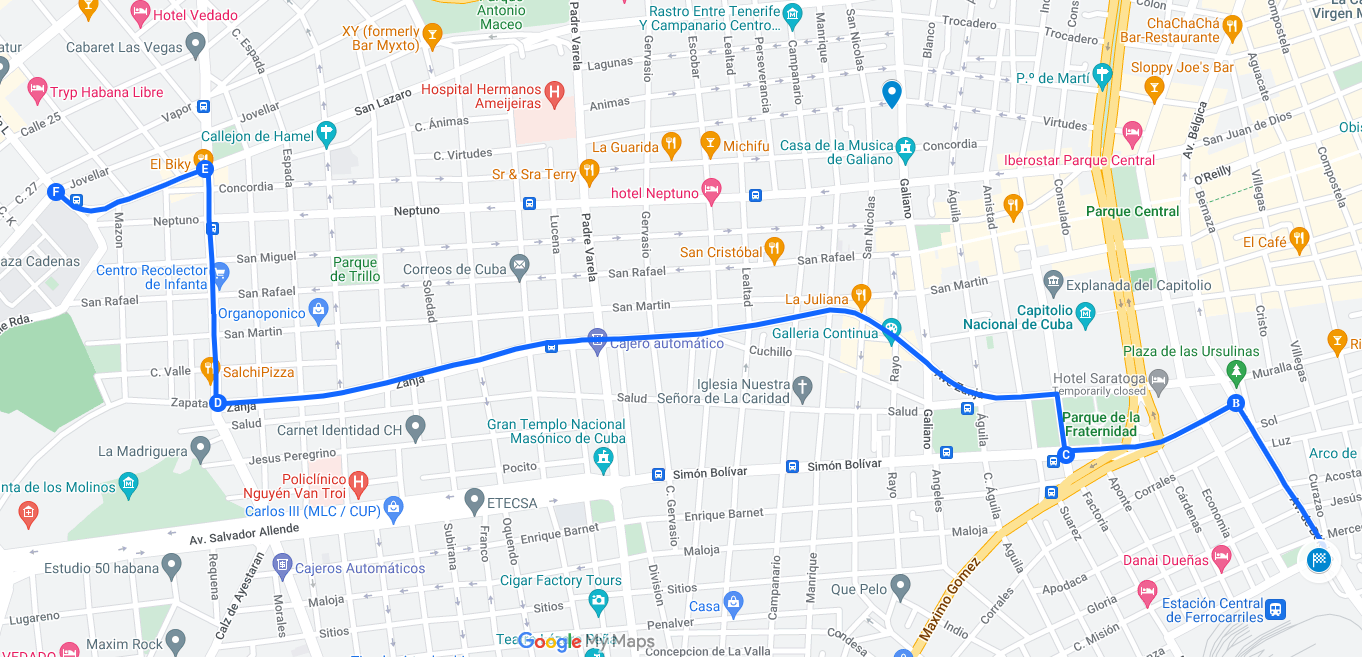
\includegraphics[scale = 0.4]{Graphics/route_3_EgidoArsenal_LyJovellarHotelColina.png}
		\caption{Ruta 3}
		\label{fig:12}
	\end{figure}

	\subsection{Detalles acerca de algunos de los baches marcados}
		En las recorridos realizados hay una gran variedad de anomalías que son baches, pero también hay muchas anomalías que, por sus características,
		son similares a un bache como, por ejemplo, una boca de alcantarilla hundida en el pavimento (ver \ref{fig:15}) que en condiciones normales no 
		tendría las mismas características (ver \ref{fig:16}). A pesar de que ambas son tapas de alcantarilla, en el primer caso las lecturas de los 
		sensores es muy probable que hayan sido similares a las de un bache.

		De igual forma, algunas otras tapas de alcantarillas no tiene las características que verdaderamente le corresponde como se puede ver en la
		figura \ref{fig:17}.

		Existen también otros objetos en la vía que no tienen las características reales y que pueden ocasionar las lecturas de los sensores sean similares
		a las de un bache como se muestra en la figura \ref{fig:18}.

		Estas anomalías que se consideraron que podían generar lecturas	similares a las de un bache se etiqutaron como tal, al igual que las anomalías que se 
		pueden apreciar en las figuras \ref{fig:19} y \ref{fig:20}, que sí son realmente baches.

\section{Los modelos de aprendizaje de máquinas}
	Luego de haber recopilado los datos con la aplicación móvil, estos fueron pasados a un programa hecho en \textbf{Python 3.10.6} con el objetivo
	de llevar a cabo la segunda fase de la propuesta. Dentro de este programa es donde se determina qué modelo de aprendizaje de máquinas se ajusta
	mejor al juego de datos, pero antes de esto fue necesario procesar los datos recolectados por la aplicación móvil y estructuralos de forma conveniente. 

	\subsection{Detalles de la estructura del juego de datos y características escogidas}
		Con el juego de datos cargado ya en el programa, se construyó un \textbf{DataFrame} de la biblioteca \textbf{pandas} donde cada columna representa
		una característica y cada fila uno de los datos recopilados. Entre las columnas de este \textbf{DataFrame} están los valores de los 3 ejes del \textbf
		{acelerómetro}, los valores de los 3 ejes del \textbf{giroscopio} y la velocidad. Estas son las primeras 7 características de nuestro juego de datos
		y son obtenidas directamente al leer los datos recopilados.\\
		\indent El resto de características son generadas a partir de las 7 previamente mencionadas y tienen como objetivo
		enriquecer el juego de datos para obtener una representación más precisa del problema que se pretende resolver. Estas características estadísticas,
		que fueron mencionadas en el capítulo anterior (ver \ref{chapter:proposal}), son computadas y agregadas como columnas al \textbf{DataFrame}.
		Luego se agregan las columnas correspondientes a la latitud, longitud y precisión de dicha ubicación, para cada uno de los datos. Finalmente, son
		eliminadas las lecturas donde la precisión es mayor que 10 metros, y se recomputa la latitud y longitud de cada dato con interpolación lineal
		utilizando la biblioteca \textbf{nvector}.

	\subsection{Detalles de la detección de anomalías}
		Una vez se tuvo el juego de datos completamente generado y refinado de acuerdo a las necesidades, se realizó un proceso de detección de anomalías.
		Para este proceso se probaron 6 métodos, 3 heurísticos y 3 métodos de aprendizaje de máquinas. Los 3 métodos heurísticos fueron los mencionados 
		en el capítulo previo (ver \ref{chapter:proposal}): \textbf{Z-Thresh}, \textbf{Z-Diff} y \textbf{G-Zero}. Con \textbf{Z-Thresh} debido a que 
		los valores de la aceleración en el eje Z se mantuvieron entre 9 y 10 mayormente (debido a la aceleración de la gravedad), se decidió escoger
		12.26 como umbral. Con \textbf{Z-Diff} se decidió escoger 4, pues en este caso lo que se intenta es detectar cambios bruscos en los valores de
		aceleración en el eje Z y en el caso de \textbf{G-Zero} se escogió 0.8 como se recomienda en la literatura\brackcite{mednis2011real}.\\
		\indent Para la detección de anomalías utilizando los métodos de aprendizaje de máquinas se utilizaron 6 de las características del \textbf
		{DataFrame}, la aceleración en los 3 ejes y la velocidad de giro en los 3 ejes. Los métodos de aprendizaje no-supervisado utilizados están
		implementados en la biblioteca \textbf{sklearn} de \textbf{Python}, específicamente en los módulos \textbf{sklearn.cluster}, donde se encuentran
		\textbf{DBSCAN} y \textbf{OPTICS}, y en \textbf{sklearn.svm}, donde se encuentra \textbf{One Class SVM}.\\
		\indent De esta forma, con cada uno de estos 6 métodos, se obtenía un \textbf{DataFrame} con los datos seleccionados como anomalías.

		Los hiperparámetros de los métodos de detección de anomalías que se probaron para determinar la mejor configuración se muestran en las tablas 
		\ref{table:4}, \ref{table:5} y \ref{table:6}.

	\subsection{Detalles del proceso de etiquetado}
		Con cada uno de los juegos de datos obtenidos por cada uno de los métodos utilizados para detectar anomalías se llevó a cabo
		el proceso de etiquetado para indentificar que anomalía es un bache. Esto, como se mencionó en el capítulo anterior(ver \ref{chapter:proposal}),
		se llevó a cabo utilizando el conjunto de marcas correspondientes a la serie temporal de la cual se extrajeron las anomalías. De esta manera, se
		le asigna una etiqueta a una anomalía indicando que es bache si existe una marca en el conjunto de marcas que se encuentre en un radio de 10
		metros. Se consideró 10 metros debido al error que mantuvo el dispositivo que se utilizó para la captura de los datos durante el proceso de
		recopilación.\\
		\indent Para computar la distancia se utilizó la fórmula de \textbf{Haversine}, que se utiliza para calcular la distancia entre dos puntos sobre la
		superficie de una esfera utilizando coordenadas de latitud-longitud. Debido a que la \textbf{Tierra} no es una esfera perfecta, tiene
		distintos radios, que van desde 6356.752 km en los polos hasta 6378.137 km en el Ecuador. A causa de esto es imposible calcular exactamente la
		distancia entre 2 puntos con esta fórmula, pero el error al hacerlo es de un 0.5\%, por lo que es bastante despreciable. El radio de la esfera
		que se consideró para este cómputo fue de 6371 km.\\

	\subsection{Detalles de la selección de características}
		Por cada juego de anomalías etiquetadas, como ya se mencionó en el capítulo previo (ver \ref{chapter:proposal}), se llevó a cabo un proceso
		de selección de características con varios métodos, para escoger cuales de estas representan mejor el problema que se pretende resolver.
		Antes de esto se eliminaron características que se consideraron no aportan información acerca de si una anomalía es bache o no como, por ejemplo,
		la velocidad, la latitud, la longitud y la precisión del \textbf{GPS}.\\
		\indent El clasificador que se utilizó para estimar dichas características en el proceso de selección fue un \emph{Random Forest}, y fue
		utilizado el que brinda el módulo \textbf{sklearn.ensembles} de la bibliotea \textbf{sklearn}. Cada vez que se corrían los métodos de selección
		de características se almacenó la información de qué características se escogieron. A dichos métodos se les pasaba el número de
		características a seleccionar. Las cantidades de características con que se probaron fueron: 3, 6 y 9.\\

	\subsection{Detalles de la selección de modelo}
		Una vez el algoritmo de selección de características terminaba, se generaba un nuevo \textbf{DataFrame} con esas únicas columnas como datos,
		y fue con este juego de datos que se pasaba a la fase de selección de modelo. En esta, se llevó a cabo un extenso proceso en el cual se buscó
		el mejor algoritmo con la mejor configuración de hiperparámetros para ese juego de datos. Los algoritmos que se probaron fueron
		mencionados en el capítulo anterior (ver \ref {chapter:proposal}).\\
		\indent Para llevar a cabo esta fase de la propuesta se utilizó la biblioteca \textbf{sklearn} de \textbf{Python}.
		Para los modelos, se utilizaron los módulos \textbf{sklearn.svm}, \textbf{sklearn.trees}, \textbf{sklearn.linear\textunderscore models},
		\textbf{sklearn. ensembles} y \textbf{sklearn.neighbors}, que permiten utilizar los métodos de aprendizaje supervisado \textbf{SVM}, \emph
		{Decision Trees}, regresión logística, \emph{Random Forest} y \textbf{KNN} respectivamente. Para separar los datos en conjunto de entrenamiento
		y de prueba se utilizó el método \textbf{train\textunderscore test\textunderscore split} del módulo \textbf{sklearn.model\textunderscore
		selection}. Se tomó como  conjunto de entrenamiento el 70\% de los datos y como conjunto de prueba el 30\%.\\
		\indent Del mismo módulo se utilizaron los objetos \textbf {RepeatedStratifiedKFold} y \textbf{GridSearchCV} para realizar validación cruzada y
		para selección de hiperparámetros respectivamente. La métrica utilizada fue \emph{F1 score}, para esto utilizamos el método \textbf{f1\textunderscore
		score} del módulo \textbf{sklearn.metrics}. De esta forma, para cada uno de los 5 métodos utilizados se pudo determinar la mejor configuración
		de hiperparámetros, realizar la validación cruzada y obtener el mejor modelo para la fase de prueba, utilizando la métrica seleccionada. A \textbf{
		RepeatedStratifiedKFold} se le pasaron argumentos para realizar 5-Fold 30 veces.

		\subsubsection{Conjuntos de hiperparámetros}
			Por cada uno de los 5 métodos utilizados, se probaron distintos conjuntos de hiperparámetros(ver figuras \ref{table:7}, \ref{table:8},
			\ref{table:9}, \ref{table:10}, \ref{table:11}). Mediante el \textbf{GridSearchCV} se buscó la mejor combinación de hiperparámetros 
			para cada uno de estos métodos.

\section{Resultados}
	En la primera fase del \emph{pipeline}, la detección de anomalías, los métodos no supervisados que mejor rendimiento mostraron en general fueron
	\textbf{DBSCAN} y \textbf{One Class SVM} como se muestra en la figura \ref{table:1}. En la tabla \ref{table:2} se pueden observar la media
	de los coeficientes de Silhouete entre todas las rutas.

	\begin{table}[htb]
		\centering
		\caption{Puntuación de Silhouete de cada algoritmo de detección de anomalías no-supervisado en cada ruta}
		\label{table:1}
		\begin{tabular}{lccc}
		\toprule
		  Ruta\textbackslash Algoritmo &    DBSCAN &     OCSVM &     OPTICS \\
		\midrule
		  Ruta1 &  0.502849 &  0.533472 &  -0.245268 \\
		  Ruta2 &  0.659878 &  0.533707 &  -0.271357 \\
		  Ruta3 &  0.620526 &  0.509438 &  -0.238291 \\
		\bottomrule
		\end{tabular}
		
	\end{table}

	\begin{table}[htb]
		\centering
		\caption{Puntuación de Silhouete media de cada algoritmo de detección de anomalías no-supervisado}
		\label{table:2}
		\begin{tabular}{lc}
		\toprule
		Algoritmo & Coeficiente de Silhouete medio \\
		\midrule
		   DBSCAN &   0.594417 	\\
		    OCSVM &   0.525539 	\\
		   OPTICS &  -0.251639 	\\
		\bottomrule
		\end{tabular}
		
	\end{table}

	Como se puede apreciar, \textbf{OPTICS} tuvo una puntuación incluso por debajo de 0, lo que indica que los \emph{clusters} se asignaron de 
	forma errónea. Por esta razón se optó por removerlo del \emph{pipeline} de la propuesta. También se recopiló información acerca de la
	cantidad de anomalías que detectó cada algoritmo(ver figura \ref{table:3}). De esta forma se pudo analizar los resultados, con lo que se decidió eliminar del \emph
	{pipeline} a \textbf{G-Zero}, pues se consideró que no detectó suficientes anomalías. Esto se supone que sea debido a que la frecuencia de
	muestreo a la que se realizaron las capturas fue demasiado baja y debido a esto no fue posible obtener los datos representativos del
	instante en el que el vehículo está en caída libre.

	\begin{table}[htb]
		\centering
		\caption{Número de anomalías detectadas por cada algoritmo}
		\label{table:3}
		\begin{tabular}{lc}
			\toprule
			 Algoritmo &  Número de Anomalías \\
			\midrule
				DBSCAN &                  134 \\
				 OCSVM &                  446 \\
				Z-Diff &                  181 \\
			   Z-Thresh &                   95 \\
				G-Zero &                    0 \\
			\bottomrule
		\end{tabular}
		
	\end{table}

	En la segunda fase del \emph{pipeline}, donde se llevó a cabo la selección de características, se pudo apreciar que ciertas características fueron
	mucho más escogidas que el resto, como fueron: 

	\begin{itemize}
		\item X / Z con 203.
		\item SpeedvsZ con 185.
		\item MeanDevGyroZ con 180.
		\item MedianDevGyroZ con 164.
	\end{itemize}

	En la tabla \ref{table:12} se puede apreciar un ranking de las 10 características más escogidas entre todas las veces que se corrió el \emph{pipeline}.

	Finalmente, en la última fase del \emph{pipeline}, se analizaron varios algoritmos de aprendizaje supervisado, con datos estandarizados y sin
	estandarizar. 
	\newpage

	En las tablas \ref{table:13}-\ref{table:16} se pueden apreciar los resultados obtenidos para cada una de las métricas, por cada algoritmo de detección de 
	anomalías utilizado.

	\begin{table}[htb]
		\centering
		\caption{Resultados usando \textbf{Z-Thresh} como método de detección de anomalías}
		\label{table:13}
		\begin{tabular}{lcccc}
		\toprule
				Model &  Accuracy &  F1 Score &  Precision &  Recall \\
		\midrule
				  KNN &    0.6897 &    0.4706 &     0.5000 &  0.4444 \\
		Random Forest &    0.6552 &    0.4444 &     0.4444 &  0.4444 \\
		Decision Tree &    0.5862 &    0.4000 &     0.3636 &  0.4444 \\
		Log Regresion &    0.7241 &    0.2000 &     1.0000 &  0.1111 \\
				  SVM &    0.6897 &    0.4706 &     0.5000 &  0.4444 \\
		\bottomrule
		\end{tabular}
	\end{table}

	\begin{table}[htb]
		\centering
		\caption{Resultados usando \textbf{Z-Diff} como método de detección de anomalías}
		\label{table:14}
		\begin{tabular}{lcccc}
		\toprule
				Model &  Accuracy &  F1 Score &  Precision &  Recall \\
		\midrule
				  KNN &    0.7455 &     0.500 &     0.5833 &  0.4375 \\
		Random Forest &    0.7818 &     0.625 &     0.6250 &  0.6250 \\
		Decision Tree &    0.6000 &     0.500 &     0.3929 &  0.6875 \\
		Log Regresion &    0.6909 &     0.320 &     0.4444 &  0.2500 \\
				  SVM &    0.7091 &     0.500 &     0.5000 &  0.5000 \\
		\bottomrule
		\end{tabular}
	\end{table}

	\begin{table}[htb]
		\centering
		\caption{Resultados usando \textbf{DBSCAN} como método de detección de anomalías}
		\label{table:15}
		\begin{tabular}{lcccc}
		\toprule
				Model &  Accuracy &  F1 Score &  Precision &  Recall \\
		\midrule
				  KNN &    0.7073 &    0.6000 &     0.6000 &  0.6000 \\
		Random Forest &    0.7805 &    0.6400 &     0.8000 &  0.5333 \\
		Decision Tree &    0.6829 &    0.6286 &     0.5500 &  0.7333 \\
		Log Regresion &    0.7073 &    0.5000 &     0.6667 &  0.4000 \\
				  SVM &    0.7073 &    0.6842 &     0.5652 &  0.8667 \\
		\bottomrule
		\end{tabular}
	\end{table}

	Las configuraciones con las que se alcanzaron estas puntuaciones se pueden ver en detalle en las tablas \ref{table:17}-\ref{table:36}.

	\newpage
	\begin{table}[htb]
		\centering
		\caption{Resultados usando \textbf{One Class SVM} como método de detección de anomalías}
		\label{table:16}
		\begin{tabular}{lcccc}
		\toprule
				Model &  Accuracy &  F1 Score &  Precision &  Recall \\
		\midrule
				  KNN &    0.7388 &    0.4262 &     0.5652 &  0.3421 \\
		Random Forest &    0.7537 &    0.2979 &     0.7778 &  0.1842 \\
		Decision Tree &    0.6791 &    0.3944 &     0.4242 &  0.3684 \\
		Log Regresion &    0.7239 &    0.2745 &     0.5385 &  0.1842 \\
				  SVM &    0.6642 &    0.3662 &     0.3939 &  0.3421 \\
		\bottomrule
		\end{tabular}
	\end{table}

	En la matriz de confusión del modelo que arrojó mejor\emph{F1 score} (ver figura \ref{fig:13}), se puede apreciar que el porcentaje de falsos
	negativos es bien bajo, lo que indica que este modelo falló en clasificar muy pocos baches. A pesar de esto, se considera que estas pruebas 
	deben ser repetidas con un conjunto de datos mucho más grande, para tener un resultado más relevante y contundente.

	\begin{figure}[htb]
		\centering
		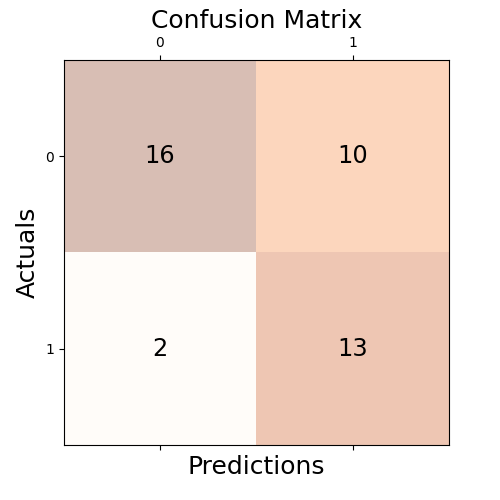
\includegraphics[scale = 0.6]{Graphics/best_model_confusion_matrix.png}
		\caption{Matriz de confusión del modelo que mejor \emph{F1 score} obtuvo.}
		\label{fig:13}
	\end{figure}

	En la siguiente imagen (figura \ref{fig:14}) se puede apreciar ubicados en un mapa con leyenda, las predicciones que realizó el modelo con mejor 
	\emph{F1 score}, en el conjunto de prueba.

	\newpage
	\begin{figure}[htb]
		\centering
		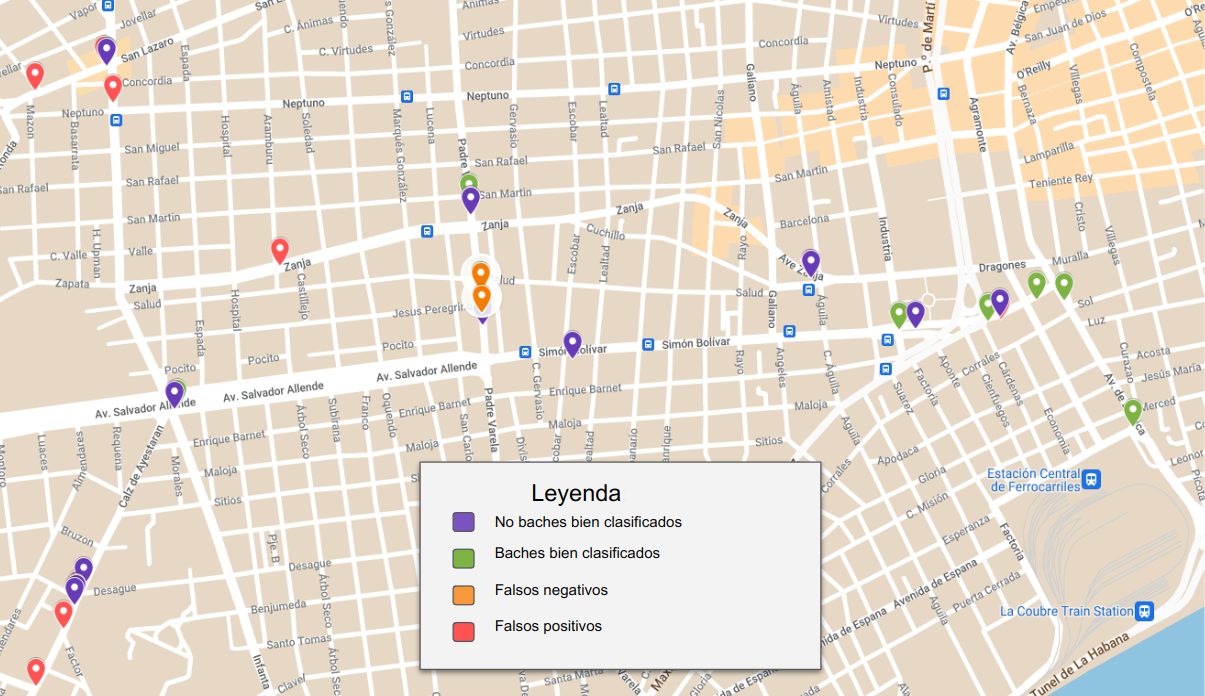
\includegraphics[scale = 0.4]{Graphics/map_point_predictions.png}
		\caption{Visualización de la ubicación de algunas de las predicciones realizadas por el modelo con mejor \emph{F1 score} en el conjunto de prueba.}
		\label{fig:14}
	\end{figure}

	La configuración con la cual se obtuvo mejores resultados utilizó \textbf{DBSCAN} para detectar las anomalías y como modelo
	supervisado \textbf{SVM}, con kernel rbf, $\gamma$ = 0.1, C = 50  y datos estandarizados. Las características seleccionadas fueron: 
	X Accel, X Gyro,  X / Z, MinZratio, MedianDevAccelY, MeanDevGyroZ. La configuración exacta con la que se obtuvo este resultado se
	puede observar en la tabla \ref{table:27}. El modelo alcanzó un \emph{F1 score} de 0.68 y un \emph{accuracy} de 0.70.


\backmatter

\begin{conclusions}
	En este trabajo se planteó como objetivo general, proponer un modelo de aprendizaje de máquinas para la detección de baches
	utilizando los sensores embebidos en los dispositivos móviles. Para esto, se implementaron 2 programas como parte de la propuesta.
	Una aplicación móvil desarrollada en \emph{Flutter} para poder obtener datos utilizando los sensores integrados de un dispositivo
	móvil. Además, se implementó un programa hecho en \emph{Python} que, utilizando los datos capturados con la aplicación, 
	permite analizar la factibilidad de un algoritmo de aprendizaje de máquinas para detectar de forma automática los baches en 
	la carretera. También fue necesario analizar el estado del arte acerca del problema de monitorear el estado de la carretera 
	utilizando sensores móviles.Esto tuvo el objetivo de determinar que sensores serían los más apropiados para resolver este problema, 
	y encontrar ideas y acercamientos previos, que pudieran servir de guía para la propuesta de solución.\\

	Se pudo comprobar el funcionamiento correcto de la aplicación móvil en varias rutas realizadas por la ciudad de La Habana y, 
	por tanto, se pudieron recopilar varios datos. Estos sirvieron luego para realizar un exhaustivo proceso, en el que los datos 
	fueron pasados a un \emph{pipeline} de 4 pasos con el cual se determinó entre varios modelos, el que mejor se ajustaba a los
	datos recopilados. Teniendo en cuenta los resultados obtenidos en este trabajo, donde se logró alcanzar un \emph{F1 score} de
	68\% y un \emph{accuracy} de 70\%, se llegó a la conclusión de que un modelo de aprendizaje de máquinas para resolver el
	problema en cuestión es factible.
\end{conclusions}

\begin{recomendations}
	Uno de los problemas con los que se tuvo que lidiar fue con la falta de datos. Por razones ajenas a la voluntad de los autores,
	entre ellas el poco tiempo con el que se contó para realizar el trabajo de campo, no se pudo recopilar un juego de datos con un 
	tamaño aceptable para los estándares requeridos por los modelos de aprendizaje de máquinas. Por esta razón, entre las propuestas
	que se considera que ayudarían mucho al proceso de recopilación de datos también está la idea de automatizar el proceso de
	etiquetado de datos. De esta forma se podría lidiar con grandes cantidades de datos, algo que es crucial para los modelos de
	aprendizaje de máquinas.

	Otra sugerencia es plantear un sistema que permita capturar las señales de los sensores sin necesidad de que
	esté fijo en una posición. Esta idea puede facilitar el uso de la aplicación para capturar los datos, incluso por personas ajenas
	al proyecto. De esta forma, cualquier persona podría ayudar a mejorar la propuesta, simplemente con utilizar la aplicación, colocarse
	el móvil en el bolsillo y montarse en cualquier vehículo para capturar datos.

	También se propone explorar el uso de técnicas de procesamiento de señales digitales que permitan mejorar la calidad de las señales
	de los sensores para obtener datos más curados e, incluso, utilizar otras características que son posibles de extraer con algunos de
	estos métodos. Otra de las ideas es explorar otras maneras de procesar las series temporales de los sensores para pasárselas a los
	modelos de aprendizaje de máquinas como, por ejemplo, analizar la serie temporal por ventanas deslizantes y tratar de encontrar los
	patrones que caracterizan el estado de la carretera. Se podría indagar, además, si existen otros sensores móviles que pudieran, de
	alguna forma, contribuir a mejorar la propuesta.

	Para futuros trabajos se propone también graficar las series temporales de los sensores en la aplicación móvil en tiempo real.
	Esto facilitaría el entendimiento del comportamiento de las señales digitales durante la captura de datos. Finalmente, como parte
	de la meta de tener una aplicación que permita monitorear el estado de la carretera se propone incorporar un \emph{backend} al
	proyecto donde los usuarios de la aplicación puedan subir los datos que hayan capturado a un servidor y, de esta forma, utilizar
	dicha información centralizada y accesible para mejorar aún más la calidad de la propuesta.
\end{recomendations}

\printbibliography[heading=bibintoc]




\end{document}
